
% ----------------------------------------------------------------------
%                   LATEX TEMPLATE FOR PhD THESIS
% ----------------------------------------------------------------------

% based on Harish Bhanderi's PhD/MPhil template, then Uni Cambridge
% http://www-h.eng.cam.ac.uk/help/tpl/textprocessing/ThesisStyle/
% corrected and extended in 2007 by Jakob Suckale, then MPI-CBG PhD programme
% and made available through OpenWetWare.org - the free biology wiki


%: Style file for Latex
% Most style definitions are in the external file PhDthesisPSnPDF.
% In this template package, it can be found in ./Latex/Classes/
\documentclass[twoside,11pt]{Latex/Classes/PhDthesisPSnPDF}


%: Macro file for Latex
% Macros help you summarise frequently repeated Latex commands.
% Here, they are placed in an external file /Latex/Macros/MacroFile1.tex
% An macro that you may use frequently is the figuremacro (see introduction.tex)
% This file contains macros that can be called up from connected TeX files
% It helps to summarise repeated code, e.g. figure insertion (see below).

% insert a centered figure with caption and description
% parameters 1:filename, 2:title, 3:description and label
\newcommand{\figuremacro}[3]{
	\begin{figure}[htbp]
		\centering
		\includegraphics[width=1\textwidth]{#1}
		\caption[#2]{\textbf{#2} - #3}
		\label{#1}
	\end{figure}
}

% insert a centered figure with caption and description AND WIDTH
% parameters 1:filename, 2:title, 3:description and label, 4: textwidth
% textwidth 1 means as text, 0.5 means half the width of the text
\newcommand{\figuremacroW}[4]{
	\begin{figure}[htbp]
		\centering
		\includegraphics[width=#4\textwidth]{#1}
		\caption[#2]{\textbf{#2} - #3}
		\label{#1}
	\end{figure}
}

% inserts a figure with wrapped around text; only suitable for NARROW figs
% o is for outside on a double paged document; others: l, r, i(inside)
% text and figure will each be half of the document width
% note: long captions often crash with adjacent content; take care
% in general: above 2 macro produce more reliable layout
\newcommand{\figuremacroN}[3]{
	\begin{wrapfigure}{o}{0.5\textwidth}
		\centering
		\includegraphics[width=0.48\textwidth]{#1}
		\caption[#2]{{\small\textbf{#2} - #3}}
		\label{#1}
	\end{wrapfigure}
}

% predefined commands by Harish
\newcommand{\PdfPsText}[2]{
  \ifpdf
     #1
  \else
     #2
  \fi
}

\newcommand{\IncludeGraphicsH}[3]{
  \PdfPsText{\includegraphics[height=#2]{#1}}{\includegraphics[bb = #3, height=#2]{#1}}
}

\newcommand{\IncludeGraphicsW}[3]{
  \PdfPsText{\includegraphics[width=#2]{#1}}{\includegraphics[bb = #3, width=#2]{#1}}
}

\newcommand{\InsertFig}[3]{
  \begin{figure}[!htbp]
    \begin{center}
      \leavevmode
      #1
      \caption{#2}
      \label{#3}
    \end{center}
  \end{figure}
}


%%% Local Variables: 
%%% mode: latex
%%% TeX-master: "~/Documents/LaTeX/CUEDThesisPSnPDF/thesis"
%%% End: 

\usepackage[T1]{fontenc}
\usepackage{array}
\usepackage{pdfpages}

%\usepackage{graphics}
% or use the graphicx package for more complicated commands
%\usepackage{graphicx}

\usepackage{nameref}

% https://www.overleaf.com/learn/latex/Code_listing
\usepackage{listings}
\usepackage{color}
\definecolor{backcolour}{rgb}{0.98, 0.98, 0.98}
\lstdefinestyle{m_style}{
    backgroundcolor=\color{backcolour},
    % commentstyle=\color{codegreen},
    % keywordstyle=\color{magenta},
    % numberstyle=\tiny\color{codegray},
    % stringstyle=\color{codepurple},
    basicstyle=\small,
    % breakatwhitespace=false,
    breaklines=true,
    % captionpos=b,
    % keepspaces=true,
    % numbers=left,
    % numbersep=5pt,
    % showspaces=false,
    % showstringspaces=false,
    % showtabs=false,     
    % tabsize=2
}
\lstset{style=m_style}

% https://tex.stackexchange.com/questions/1601/replacing-itemize-by-mdwlists-itemize-throughout
\usepackage{mdwlist}
\let\stditemize\itemize
\let\endstditemize\enditemize
\let\itemize\undefined
\makecompactlist{itemize}{stditemize}


%: ----------------------------------------------------------------------
%:                  TITLE PAGE: name, degree,..
% ----------------------------------------------------------------------
\usepackage{graphicx}

      \textwidth 15cm
      \textheight 22cm
      \parindent 10pt
      \oddsidemargin 0.85cm
      \evensidemargin 0.37cm


\begin{document}

\thispagestyle{empty}

\begin{center}

Vrije Universiteit Amsterdam \hspace*{2cm} Universiteit van Amsterdam

\vspace{1mm}

\hspace*{-7.5cm}
\includegraphics[height=25mm]{0_frontmatter/figures/vu-griffioen.pdf}

\vspace*{-2cm}\hspace*{7.5cm}
\includegraphics[height=15mm]{0_frontmatter/figures/uva_logo.jpg}

\vspace{2cm}

{\Large Master Thesis}

\vspace*{1.5cm}

\rule{.9\linewidth}{.6pt}\\[0.4cm]
{\huge \bfseries Title of the Thesis\par}\vspace{0.4cm}
\rule{.9\linewidth}{.6pt}\\[1.5cm]

\vspace*{2mm}

{\Large
\begin{tabular}{l}
{\bf Author:} ~~student name ~~~~ (student number)
\end{tabular}
}

\vspace*{2cm}

\begin{tabular}{ll}
{\it 1st supervisor:}   & ~~supervisor name \\
{\it daily supervisor:} & ~~supervisor name ~~~~ (company, if applicable) \\
{\it 2nd reader:}       & ~~supervisor name
\end{tabular}

\vspace*{2.5cm}

\textit{A thesis submitted in fulfillment of the requirements for\\ the joint UvA-VU Master of Science degree in Computer Science}

\vspace*{1.8cm}

\today\\[4cm] % Date

\end{center}

\newpage


% ----------------------------------------------------------------------
       
% turn of those nasty overfull and underfull hboxes
\hbadness=10000
\hfuzz=50pt


%: --------------------------------------------------------------
%:                  FRONT MATTER: dedications, abstract,..
% --------------------------------------------------------------


%\language{english}


% sets line spacing
\renewcommand\baselinestretch{1.2}
\baselineskip=18pt plus1pt


%: ----------------------- generate cover page ------------------------

\begin{center}
\textit{``I am the master of my fate, I am the captain of my soul'' \\ from {\em Invictus}, by William Ernest Henley}
\end{center}

%: ----------------------- cover page back side ------------------------
% Your research institution may require reviewer names, etc.
% This cover back side is required by Dresden Med Fac; uncomment if needed.

\newpage
%\vspace{10mm}
%1. First Reader: Name Surname
%
%\vspace{10mm}
%2. Daily Supervisor: Name Surname
%
%\vspace{10mm}
%3. Second Reader: Name Surname
%
%\vspace{10mm}
%4. Industrial Supervisor: Name Surname
%
%\vspace{20mm}
%Day of the defense:

%\vspace{20mm}
%\hspace{70mm}Signature from head of PhD committee:



%: ----------------------- abstract ------------------------

% Your institution may have specific regulations if you need an abstract and where it is to be placed in the document. The default here is just after title.


% Thesis Abstract -----------------------------------------------------


%\begin{abstractslong}    %uncommenting this line, gives a different abstract heading
\begin{abstracts}        %this creates the heading for the abstract page

Existing columnar database systems rely on a small set of lightweight compression techniques to achieve smaller data size and fast query execution: RLE, DICT, FOR, DELTA and their improved versions. These are hardcoded blackbox approaches with limited capacity of exploiting all compression opportunities present in real data. We propose \textit{whitebox compression}: a new compression model which represents data through elementary operator expressions automatically generated at bulk load. This is done by learning patterns from the data and associating them with operators to form expression trees, which are stored together with the compressed data and lazily evaluated during query execution. \textit{Whitebox compression} automatically finds and exploits compression opportunities, leading to transparent, recursive and more compact representations of the data. Combined with vectorized execution or JIT code generation, it has the potential to generate powerful compression schemes in terms of both compression ratio and query execution time. Our focus is on real data rather than synthetic datasets, thus we develop and evaluate the \textit{whitebox compression} model using the Public BI benchmark---a comprehensive human generated benchmark for database systems.
\end{abstracts}
%\end{abstractlongs}


% ---------------------------------------------------------------------- 


% The original template provides and abstractseparate environment, if your institution requires them to be separate. I think it's easier to print the abstract from the complete thesis by restricting printing to the relevant page.
% \begin{abstractseparate}
%   
% Thesis Abstract -----------------------------------------------------


%\begin{abstractslong}    %uncommenting this line, gives a different abstract heading
\begin{abstracts}        %this creates the heading for the abstract page

Existing columnar database systems rely on a small set of lightweight compression techniques to achieve smaller data size and fast query execution: RLE, DICT, FOR, DELTA and their improved versions. These are hardcoded blackbox approaches with limited capacity of exploiting all compression opportunities present in real data. We propose \textit{whitebox compression}: a new compression model which represents data through elementary operator expressions automatically generated at bulk load. This is done by learning patterns from the data and associating them with operators to form expression trees, which are stored together with the compressed data and lazily evaluated during query execution. \textit{Whitebox compression} automatically finds and exploits compression opportunities, leading to transparent, recursive and more compact representations of the data. Combined with vectorized execution or JIT code generation, it has the potential to generate powerful compression schemes in terms of both compression ratio and query execution time. Our focus is on real data rather than synthetic datasets, thus we develop and evaluate the \textit{whitebox compression} model using the Public BI benchmark---a comprehensive human generated benchmark for database systems.
\end{abstracts}
%\end{abstractlongs}


% ---------------------------------------------------------------------- 

% \end{abstractseparate}


%: ----------------------- tie in front matter ------------------------

\frontmatter
% Thesis Dedication ---------------------------------------------------

%\begin{dedication} %this creates the heading for the dedication page

%To ...

%\end{dedication}

% ----------------------------------------------------------------------
% Thesis Acknowledgements ------------------------------------------------


%\begin{acknowledgementslong} %uncommenting this line, gives a different acknowledgements heading
%\begin{acknowledgements}      %this creates the heading for the acknowlegments


%\end{acknowledgements}
%\end{acknowledgmentslong}

% ------------------------------------------------------------------------





%: ----------------------- contents ------------------------

\setcounter{secnumdepth}{3} % organisational level that receives a numbers
\setcounter{tocdepth}{3}    % print table of contents for level 3
\tableofcontents            % print the table of contents
% levels are: 0 - chapter, 1 - section, 2 - subsection, 3 - subsection


%: ----------------------- list of figures/tables ------------------------

\listoffigures	% print list of figures

\listoftables  % print list of tables




%: ----------------------- glossary ------------------------

% Tie in external source file for definitions: /0_frontmatter/glossary.tex
% Glossary entries can also be defined in the main text. See glossary.tex
% 
%% this file is called up by thesis.tex
% content in this file will be fed into the main document

% Glossary entries are defined with the command \nomenclature{1}{2}
% 1 = Entry name, e.g. abbreviation; 2 = Explanation
% You can place all explanations in this separate file or declare them in the middle of the text. Either way they will be collected in the glossary.

% required to print nomenclature name to page header
%\markboth{\MakeUppercase{\nomname}}{\MakeUppercase{\nomname}}


% ----------------------- contents from here ------------------------


%\nomenclature{LSY}{ehbfuefebbfbjkjkebfjbfbfw} 
%\nomenclature{DEPC}{diethyl-pyro-carbonate; used to remove RNA-degrading enzymes (RNAases) from water and laboratory utensils}
%\nomenclature{DMSO}{dimethyl sulfoxide; organic solvent, readily passes through skin, cryoprotectant in cell culture}
%\nomenclature{EDTA}{Ethylene-diamine-tetraacetic acid; a chelating (two-pronged) molecule used to sequester most divalent (or trivalent) metal ions, such as calcium (Ca$^{2+}$) and magnesium (Mg$^{2+}$), copper (Cu$^{2+}$), or iron (Fe$^{2+}$ / Fe$^{3+}$)}



 

%\begin{multicols}{2} % \begin{multicols}{#columns}[header text][space]
%\begin{footnotesize} % scriptsize(7) < footnotesize(8) < small (9) < normal (10)

%\printnomenclature[1.5cm] % [] = distance between entry and description
%\label{nom} % target name for links to glossary

%\end{footnotesize}
%\end{multicols}



%: --------------------------------------------------------------
%:                  MAIN DOCUMENT SECTION
% --------------------------------------------------------------

% the main text starts here with the introduction, 1st chapter,...
\mainmatter

\renewcommand{\chaptername}{} % uncomment to print only "1" not "Chapter 1"


%: ----------------------- subdocuments ------------------------

% Parts of the thesis are included below. Rename the files as required.
% But take care that the paths match. You can also change the order of appearance by moving the include commands.

% this file is called up by thesis.tex
% content in this file will be fed into the main document

%: ----------------------- introduction file header -----------------------
\chapter{Introduction}

% ----------------------- paths to graphics ------------------------

\graphicspath{{1_introduction/images/}}

% ----------------------- contents from here ------------------------
%


% \section{Context and motivation}

This thesis presents a new compression model for columnar database systems: \emph{whitebox compression}. Existing DBMSs use compression to make data smaller in terms of disk space, respectively to make queries faster by reducing I/O and memory usage and operating on the compressed data directly, without decompression. State-of-the-art columnar compression methods may not exploit all opportunities offered by the data, e.g. because these methods (RLE, FOR, DICT, DELTA) work on only one column at a time and hence cannot exploit correlations between multiple columns. Another reason is that users often use "sub-optimal" datatypes to represent their data, e.g. storing dates or numbers in strings, which are harder to compress and more expensive to operate on. Achieving high compression ratios is an important factor that influences the ability of DBMSs to scale up in terms of storage space. Compressed data leads to reducing the I/O bottleneck between disk and main memory and even between main memory and CPU if done at a granular level \cite{zukowski2006super}. Moreover, higher computation efficiency can be achieved through compression, since operating over thinner data optimizes the use of SIMD instructions.

Actual data found in real datasets tends to exhibit phenomena not found in synthetic database benchmarks like TPC-H \cite{boncz2013tpc} and TPC-DS \cite{nambiar2006making}. Not only is data often skewed in terms of value and frequency distribution, but it is also correlated across columns. Our recent efforts led to the first fully user-generated benchmark for database systems: the Public BI benchmark \cite{pbib}. Its many human-generated datasets and real data distributions open new grounds for research in the direction of columnar data compression and compressed execution. Our goal is to leverage the characteristics of these datasets for finding new methods of compression which perform well on real data rather than synthetic benchmarks. We believe the best way to achieve this is through \emph{whitebox compression}: using basic operators to create expression trees that enable efficient processing of the data.

% Existing compression methods fail to identify all compression possibilities that may exist in real data, as well as opportunities to operate directly on compressed data by pushing predicates down. We believe that, having a user-generated dataset is the perfect opportunity to learn more about real data. The goal is to find a better representation for it, which will lead to a better compression ratio and more opportunities for executing queries directly on compressed data.

% \textit{Whitebox compression} requires high performance expression evaluation provided only by modern techniques like vectorized execution or JIT code generation. These systems have so far confined themselves to the blackbox approach of only supporting a few hard-coded compression methods such as RLE, DICT, FOR and DELTA. Moreover, the problem of choosing the compression expression is workload dependent, as different data distributions and patterns can be better represented only by using dedicated combinations of operators.

% ------------ whitebox compression ------------ %

\section{Whitebox compression}

\textit{Whitebox compression} is a compression model for database systems that represents data through an expression language composed of elementary operators. Multiple operators are chained together to form an expression tree where inner nodes are operators and leaves are physical columns. A physical column is the partial representation of a logical column used for storage on disk. A logical column is the data as seen by the user. The evaluation of an expression tree on the physical columns generates the original logical columns. 

Take for example, a logical column \verb|A| which stores email addresses. It can be split by the \verb|'@'| character into 2 new columns \verb|A1| and \verb|A2|. The first one will contain the local/username part of the email address and the second one its domain (e.g. for \verb|"john.smith@gmail.com"| \verb|A1| will store \verb|"john.smith"| and \verb|A2| will store \verb|"@gmail.com"|). The second column will then be compressed with dictionary encoding to exploit the small number of unique email address domains. Stored together, email addresses are not compressible because of the uniqueness of the usernames. Through \textit{whitebox} representation, subparts of the data can be compressed independently.

\begin{figure}[h]
  \centering
  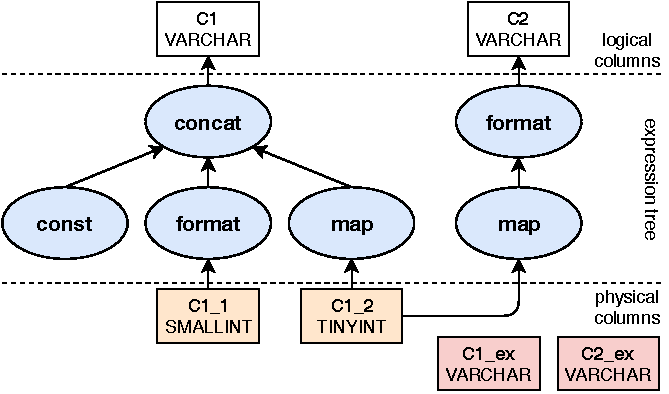
\includegraphics[width=0.75\linewidth]{intro-example_1.pdf}
  \caption{Whitebox representation example}
  \label{fig:intro:whitebox:example}
\end{figure}

Figure~\ref{fig:intro:whitebox:example} illustrates the general concept of \textit{whitebox compression}. \verb|C1| and \verb|C2| are 2 logical columns represented through elementary operator expressions as functions of the physical columns \verb|C1_1| and \verb|C1_2|. The operators are, in this example: \verb|concat|, \verb|format|, \verb|map| and \verb|const|. Chained together, they form \textit{expression trees} that transparently describe the columnar transformations applied to the data. Values that do not match the expressions are stored in the exception columns \verb|C1_ex| and \verb|C2_ex|.

The \textit{whitebox} representation creates compression opportunities. While in the original format, columns cannot be compressed through existing lightweight techniques, the physical columns resulting after applying the operator expressions are storing data more compactly. E.g. string columns are decomposed into subcolumns based on the different distributions of substring components and redundancy is eliminated by representing correlated columns as functions of the same physical columns. This process leads to efficient representation of the data in columns with appropriate datatypes and sparse exception columns.

% TODO: different example here.
% Another example is the logical column "customer\_id" with values of the following format: "customer\_no\_\$\{x\}", where \$\{x\} is a fixed length 6 digit integer (e.g. "customer\_no\_000001", "customer\_no\_000736", etc.). We can represent this column through the expression: \emph{format("customer\_no\_\%06d", delta\_inv(\$\{x\}))}. Here we have the \emph{format} operator which takes as parameter a format string similar to the \emph{printf} function in C. The second operator is \emph{delta\_inv}, meaning the decompression function for DELTA. The corresponding compression tree is depicted in Figure \ref{fig:intro:whitebox:example}.

% In both examples the data is transformed in a way that creates compression opportunities. While in the original format the data cannot be compressed through lightweight techniques, the columns resulting after applying the operators are either reduced to a single value ("customer\_no\_") or compressed with DELTA or DICT.

The difference between \textit{blackbox compression} and \textit{whitebox compression} is best perceived from the system's perspective. Table~\ref{tab:intro:blackboxwhitebox} shows a comparison between the 2 models.

\begin{table}[h]
\centering
\makebox[\textwidth][c]{
\begin{tabular}{l|l|l}
                    & \multicolumn{1}{c|}{Blackbox} & \multicolumn{1}{c}{Whitebox}          \\ \hline
Nature              & hardcoded, opaque             & generic, flexible, transparent        \\
Header info & identifier (e.g. PFOR)        & operator expression, self-descriptive \\
Output              & block of data                 & columns (allows recursion)            \\
Exceptions          & included in the data block    & separate columns                     
\end{tabular}
}
\caption{Blackbox vs. whitebox comparison}
\label{tab:intro:blackboxwhitebox}
\end{table}

A \textit{blackbox compression} system takes as input a column and outputs a block of data, containing both the compressed values and the exceptions, stored in a format only known by the system. In contrast, a \textit{whitebox compression} system takes as input a set of columns and outputs an expression tree and other columns. The representation of the columns is transparent and self-descriptive, which enables  partial decompression of the data by pushing operators down the compression tree at query execution time. The \textit{whitebox compression} model is generic and flexible, allowing recursive compression of columns---including exceptions. It can be easily extended with new operators and adapted according to the system's needs and data characteristics.

\iffalse
- distinction between whitebox and blackbox compression/representation
- see presentation slides
\fi

% ------------ research questions ------------ %

% \newpage
\section{Research questions}

The goal of our project is to explore the concept of \emph{whitebox compression} with the purpose of finding a better way to compress human-generated data. To this end, we defined a list of scientific questions that we answer during our research.
\begin{enumerate}[1)]
    \item What does real, user-generated data look like---specifically in the case of the Public BI benchmark?
    \begin{enumerate}[a)]
        \item What patterns can we find in the columns of each dataset?
        \item Inefficient ways of representing data?
        \item "Wrong" type used to define data (e.g. number stored as string, etc.)?
    \end{enumerate}
    \item How good are existing compression schemes at compressing real data?
    \begin{enumerate}[a)]
        \item Do they make the most out of the properties of the data?
        \item Is there room for improvement?
    \end{enumerate}
    \item Can we represent the logical columns more compactly through an expression tree composed of elementary operators?
    \begin{enumerate}[a)]
        \item What kind of operators are suitable for expressing the data and transforming it to physical columns?
        \item What will the compression ratio be?
        \item Can we exploit correlations between multiple logical columns by sharing the physical columns in their expressions?
    \end{enumerate}
    \item Can we create an automatic learning process that will generate suitable compression trees for each column?
    \begin{enumerate}[a)]
        \item Will it provide a high compression ratio?
        \item How will it compare to existing solutions?
    \end{enumerate}
\end{enumerate}

The focus of this thesis is on learning patterns from the data and automatically generating expression trees for more compact data representation---everything optimized for size. An additional, but equally important aspect of this topic is query execution time and whether it can be improved through \textit{whitebox compression}. We leave this subject for future work. We defined the corresponding research question below for completeness, but we do not answer it in this thesis. 
\begin{enumerate}[1)]
    \setcounter{enumi}{4}
    \item Can we achieve compressed execution with the \textit{whitebox compression} model?
    \begin{enumerate}[a)]
        \item Can we exploit SIMD in the scan?
        \item Will there be lazy decompression opportunities?
        \item Can we push query predicates down the compression tree?
    \end{enumerate}
\end{enumerate}

We carried out our research and structured this thesis according to these questions. We present related work in Chapter~\ref{ch:relatedwork}. We performed a characterisation of the Public BI benchmark and then manually analyzed its datasets in search for patterns and compression opportunities not exploited by the existing systems (Chapter~\ref{ch:pbib}). Based on our findings, we defined the \textit{whitebox compression} model, the expression language and all its characteristics in Chapter~\ref{ch:exprlang}. Furthermore, we defined algorithms that automatically detect compression opportunities and generate compression trees that represent data more compactly (Chapter~\ref{ch:automaticlearning}). Finally, we evaluate our proof-of-concept implementation of \textit{whitebox compression} against an existing database system and an estimator model baseline (Chapter~\ref{ch:evaluation}).


% this file is called up by thesis.tex
% content in this file will be fed into the main document

\chapter{Related work}
\label{ch:relatedwork}


% ----------------------- paths to graphics ------------------------

% change according to folder and file names
\ifpdf
    \graphicspath{{7/figures/PNG/}{7/figures/PDF/}{7/figures/}}
\else
    \graphicspath{{7/figures/EPS/}{7/figures/}}
\fi


% ----------------------- contents from here ------------------------
% 

The topic of data compression has received significant attention from the database research community over the past 25 years \cite{abadi2006integrating,zukowski2006super,lang2016data,polychroniou2015efficient,graefe1991data}. Existing work covers a wide range of approaches to this problem: compression algorithms, efficient hardware-conscious implementations, compressed execution, all integrated into real database systems \cite{kemper2011hyper,zukowski2012vectorwise}.

The goal of reducing I/O bandwidth has directed the focus towards lightweight compression schemes: dictionary compression, run-length encoding, frame-of-reference, delta coding, null suppression \cite{abadi2006integrating,goldstein1998compressing,lemire2015decoding,roth1993database,zukowski2006super}. Zukowski et al. \cite{zukowski2006super} proposed improved versions of these techniques that efficiently handle exceptions---making the compression methods less vulnerable to outliers---and achieve fast vectorized execution. Various storage formats that facilitate compression and compressed execution have been proposed. Data Blocks \cite{lang2016data} is a compressed columnar storage format that reduces the memory footprint through hot-cold data classification. Raman et al. \cite{raman2013db2} optimized query execution time for analytics use cases through in memory query processing on the dictionary compressed column-organized format of IBM DB2 BLU.

All this work focuses on low level optimizations to either speed up query execution or improve the compression rates. These solutions revolve around the same compression schemes and rely on fine-tuned hardware-conscious implementations leveraging SIMD instructions and vectorized execution to save CPU cycles and increase CPU efficiency. In contrast, we approach the problem of compression from a different angle. Our focus is on expressing the data in a completely different way, through simple operators chained together to form data-aware compression trees. Automatic generation of these compression expressions is based on finding patterns in the data and correlations amongst different columns. Lee et al. \cite{lee2014joins} mention the possibility of exploiting the correlations among columns at query time with the purpose of performing join operations on columns with different encodings. In contrast, we want to exploit these correlations during compression, to obtain better compression ratios.

The closest work to our research is \cite{raman2006wring}, where Raman et al. exploit data properties (skewed distributions and correlations) to achieve high compression ratios. They concatenate correlated columns and encode them together using a variation of Huffman trees which preserve partial ordering. Additionally, a sequence of type specific transformations, sorting and delta coding is also applied. We see this approach as heavy-weight black-box compression as it is hard-coded and relies on multiple rounds of Huffman encoding. Moreover, all the patterns in the data need to be manually supplied by the user (correlations and domain specific transformations). Our work differs in multiple ways: 1) we exploit correlated columns by sharing the same physical columns between related logical columns; 2) we apply a wide range of domain specific operators tailored to the data, including splitting columns and then recursively applying the same procedure; 3) our process is fully automated, from determining patterns and correlations between columns, to generating custom expressions trees.

Damme et al. \cite{damme2017lightweight} performed an exhaustive evaluation of existing compression algorithms and concluded that compression rates are highly dependent on the properties of the data and that combinations of multiple techniques lead to the best results. These results support our reasons for better understanding the data and chaining elementary operators into complex compression trees and encourage us to see how our \textit{whitebox} approach affects both compression rates and query execution time.

Additionally, while most compression solutions proposed so far were mainly evaluated and compared to each other on synthetic benchmarks \cite{abadi2006integrating,zukowski2006super,lee2014joins,lang2016data,raman2013db2}, we are the first to use such a comprehensive human-generated benchmark as the Public BI benchmark \cite{pbib}---which we defined as an early stage of this research project and will be described in more depth in the next chapter. Two examples of benchmarks used for evaluating database compression and compressed execution are TPC-H \cite{boncz2013tpc} and its successor TPC-DS \cite{nambiar2006making}. Both are synthetic, using uniform or stepwise uniform column value distributions, with fully independent columns in and between tables. This absence of skew, data dirtiness and correlation does not reflect the nature of real data. In contrast, the Public BI benchmark contains 386 GB of real data and 646 analytics queries available on Tableau Public \cite{vogelsgesang2018get, tableaupublic}. The large volume of data, it’s diversity in content and the extended character set make it suitable for evaluating compression solutions. It is an open-source benchmark and we hope it will be useful to the database community in many ways.

% ------------ contributions ------------ %

\section{Contributions}

This thesis brings the following contributions:
\begin{enumerate}[1)]
\item Public BI benchmark analysis---an analysis of real, user-generated data from the perspective of compression
\item \textit{whitebox compression}---a new generic, extensible, recursive and transparent compression model for columnar databases, which achieves higher compression ratios by representing data more compactly through elementary operator expressions and creates opportunities for faster query execution
\item \textit{learned compression}---automatic identification of patterns in the data and generation of compression trees: multiple pattern detectors, a cost model and compression learning algorithms
\end{enumerate}

% Our work will consist in defining, implementing and evaluating a \emph{whitebox compression} framework. We will invent an expression language and \emph{learn} expressions from the data during bulk loading. To achieve this we will need to overcome multiple challenges.

% The first challenge is finding the characteristics of our dataset that makes it different from synthetic data. While generating table-level statistics is trivial, we need to go further and determine common patterns that can benefit from compression, find suitable operators and combine them to form expressions (compression trees). Moreover, these expressions should facilitate compressed execution.

% A second challenge will be to automatically learn and generate the best compression tree for each column, while data is loaded or inserted. We expect to find values that do not comply to the patterns we want to exploit (i.e. exceptions from the rule). We will need to find ways to efficiently deal with these exceptions, in terms of writing them to disk without affecting the compression ratio and reading them back without impacting query execution time.



% ---------------------------------------------------------------------------
% ----------------------- end of thesis sub-document ------------------------
% ---------------------------------------------------------------------------

% this file is called up by thesis.tex
% content in this file will be fed into the main document

\chapter{Public BI benchmark} % top level followed by section, subsection
\label{ch:pbib}

% ----------------------- paths to graphics ------------------------

\graphicspath{{3_pbib/images/}}

% ----------------------- contents from here ------------------------
% 

The Public BI benchmark \cite{pbib} is a user-generated benchmark for database systems derived from the DBTest'18 paper by Tableau \cite{vogelsgesang2018get}. It contains 386GB of real data and 646 analytics queries, available at \url{https://github.com/cwida/public_bi_benchmark} under the MIT License. The data distributions, diversity in content and the extended character set make it suitable for evaluating compression solutions.

The benchmark was created by downloading 46 of the biggest workbooks from Tableau Public \cite{tableaupublic} and converting the data to CSV files. The SQL queries were collected from the Tableau logs that appear when visualizing the workbooks (SQL queries to the integrated HyPer \cite{kemper2011hyper} engine). We processed the CSV files with the purpose of making them load into different database systems. The queries contained Tableau-specific functions and syntax. We processed and adapted them in order to run on MonetDB \cite{boncz2005monetdb} and VectorWise \cite{zukowski2012vectorwise}. Table~\ref{tab:pbib:workbooks} shows a summary of the benchmark.
% The presentation of the Public BI benchmark creation process is not in the scope of this thesis and will not be further discussed here.

% TODO-1: document the creation process in the appendix (if there is time)

This chapter presents a characterisation of the Public BI benchmark that we performed with the purpose of understanding what real data looks like and finding opportunities for more compact data representation. This analysis was performed solely from the perspective of compression. We did not analyze entities, relationships or the queries.

\begin{table}[!h]
\centering
\singlespacing
\small
\begin{tabular}{@{}l|ccccc@{}}
\toprule
Workbook & Tables & Columns & Rows & Queries & CSV size \\ \midrule
Arade & 1 & 11 & 9.9M & 1 & 811.4MiB \\
Bimbo & 1 & 12 & 74.2M & 2 & 3.0GiB \\
CMSprovider & 2 & 52 & 18.6M & 3 & 3.9GiB \\
CityMaxCapita & 1 & 31 & 912.7K & 10 & 333.0MiB \\
CommonGovernment & 13 & 728 & 141.1M & 38 & 102.5GiB \\
Corporations & 1 & 27 & 741.7K & 1 & 202.2MiB \\
Eixo & 1 & 80 & 7.6M & 24 & 6.4GiB \\
Euro2016 & 1 & 11 & 2.1M & 1 & 390.6MiB \\
Food & 1 & 6 & 5.2M & 1 & 205.9MiB \\
Generico & 5 & 215 & 114.1M & 38 & 64.5GiB \\
HashTags & 1 & 101 & 511.5K & 12 & 640.2MiB \\
Hatred & 1 & 31 & 873.2K & 26 & 309.4MiB \\
IGlocations1 & 1 & 18 & 81.6K & 3 & 6.6MiB \\
IGlocations2 & 2 & 40 & 4.3M & 13 & 1.8GiB \\
IUBLibrary & 1 & 27 & 1.8K & 3 & 443.3KiB \\
MLB & 68 & 3733 & 32.5M & 95 & 8.2GiB \\
MedPayment1 & 1 & 28 & 9.2M & 1 & 1.7GiB \\
MedPayment2 & 1 & 29 & 9.2M & 1 & 1.8GiB \\
Medicare1 & 2 & 52 & 17.3M & 10 & 3.3GiB \\
Medicare2 & 2 & 56 & 18.3M & 9 & 3.4GiB \\
Medicare3 & 1 & 29 & 9.3M & 1 & 2.1GiB \\
Motos & 2 & 88 & 28.4M & 24 & 16.1GiB \\
MulheresMil & 1 & 81 & 7.6M & 35 & 6.4GiB \\
NYC & 2 & 108 & 19.2M & 5 & 12.6GiB \\
PanCreactomy1 & 1 & 29 & 9.2M & 2 & 2.0GiB \\
PanCreactomy2 & 2 & 58 & 18.3M & 11 & 4.1GiB \\
Physicians & 1 & 28 & 9.2M & 1 & 1.7GiB \\
Provider & 8 & 224 & 73.2M & 46 & 13.6GiB \\
RealEstate1 & 2 & 56 & 39.1M & 9 & 10.6GiB \\
RealEstate2 & 7 & 189 & 66.4M & 23 & 17.1GiB \\
Redfin1 & 4 & 176 & 12.1M & 5 & 5.3GiB \\
Redfin2 & 3 & 132 & 9.1M & 4 & 4.0GiB \\
Redfin3 & 2 & 94 & 6.5M & 3 & 3.0GiB \\
Redfin4 & 1 & 48 & 3.3M & 2 & 1.5GiB \\
Rentabilidad & 9 & 1266 & 3.6M & 35 & 3.3GiB \\
Romance & 2 & 24 & 3.2M & 3 & 1.0GiB \\
SalariesFrance & 13 & 695 & 16.2M & 32 & 12.6GiB \\
TableroSistemaPenal & 8 & 174 & 25.3M & 23 & 5.3GiB \\
Taxpayer & 10 & 280 & 91.5M & 22 & 17.1GiB \\
Telco & 1 & 181 & 2.9M & 1 & 2.3GiB \\
TrainsUK1 & 4 & 87 & 12.9M & 8 & 3.9GiB \\
TrainsUK2 & 2 & 74 & 31.1M & 1 & 12.2GiB \\
USCensus & 3 & 1557 & 9.4M & 8 & 13.6GiB \\
Uberlandia & 1 & 81 & 7.6M & 24 & 6.4GiB \\
Wins & 4 & 2198 & 2.1M & 13 & 3.9GiB \\
YaleLanguages & 5 & 150 & 5.8M & 13 & 1.5GiB \\ \midrule
Total & 206 & 13395 & 988.9M & 646 & 386.5GiB \\ \bottomrule
\end{tabular}
\caption{Public BI benchmark workbooks}
\label{tab:pbib:workbooks}
\end{table}
\FloatBarrier

\section{Benchmark analysis}
\label{sec:pbib:characterisation}

\subsection{General characterisation}

We started by analyzing the tables in terms of number or rows, columns and size. Figure~\ref{fig:pbib:generalstats} shows the distribution of these metrics over the tables. 40\% of the tables have less than 1 million rows and 50\% of the tables have between 1 and 10 million rows. 90\% of the tables have less than 80 columns. In terms of size, the majority of the tables have less than 3GB (uncompressed), but there are also larger tables, up to 14GB.

\begin{figure}[h]
\centering
\makebox[\textwidth][c]{
\begin{subfigure}[t]{0.35\linewidth}
  \centering
  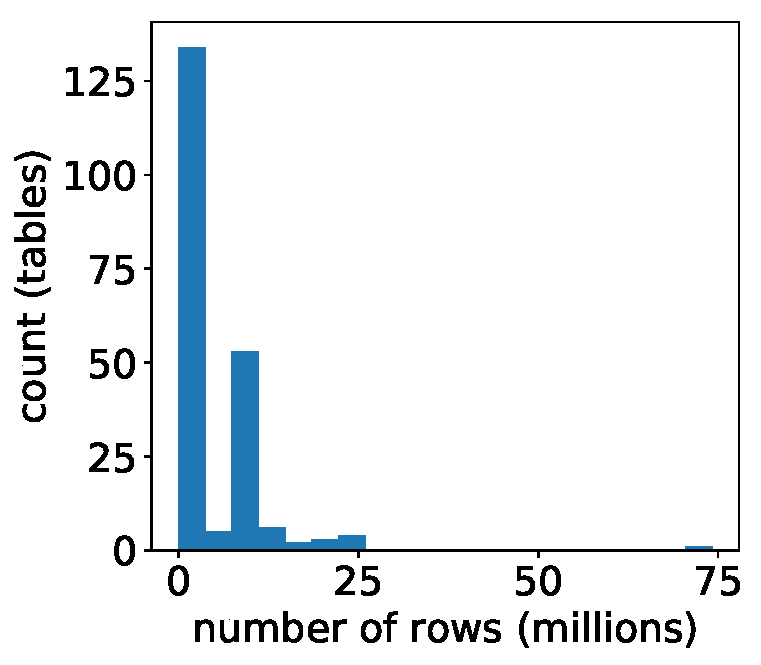
\includegraphics[width={1.0\linewidth}]{rows.pdf}
  \caption{Row distribution}
  \label{fig:pbib:generalstats:rows}
\end{subfigure}
% \hspace{1em}
\begin{subfigure}[t]{0.35\linewidth}
  \centering
  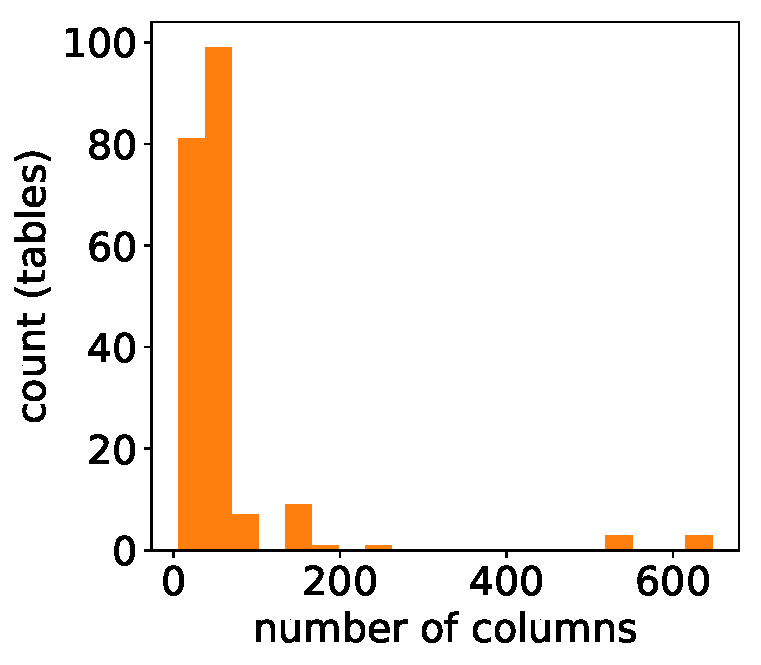
\includegraphics[width={1.0\linewidth}]{column_count.pdf}
  \caption{Column distribution}
  \label{fig:pbib:generalstats:columns}
\end{subfigure}
% \hspace{1em}
\begin{subfigure}[t]{0.35\linewidth}
  \centering
  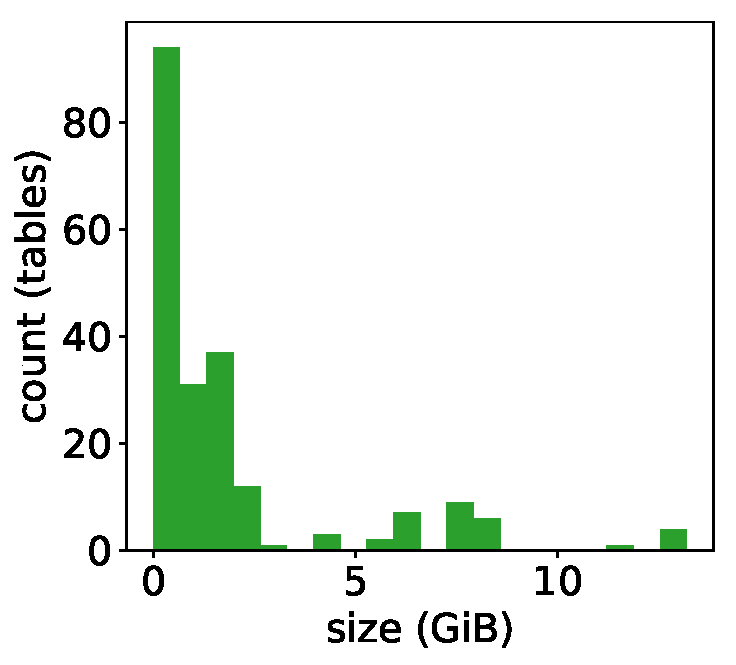
\includegraphics[width={1.0\linewidth}]{size_csv.pdf}
  \caption{Data size distribution}
  \label{fig:pbib:generalstats:size}
\end{subfigure}
}
\caption{Row, column and size distribution}
\label{fig:pbib:generalstats}
\end{figure}

\begin{figure}[h]
\centering
\makebox[\textwidth][c]{
\begin{subfigure}[t]{0.55\linewidth}
  \centering
  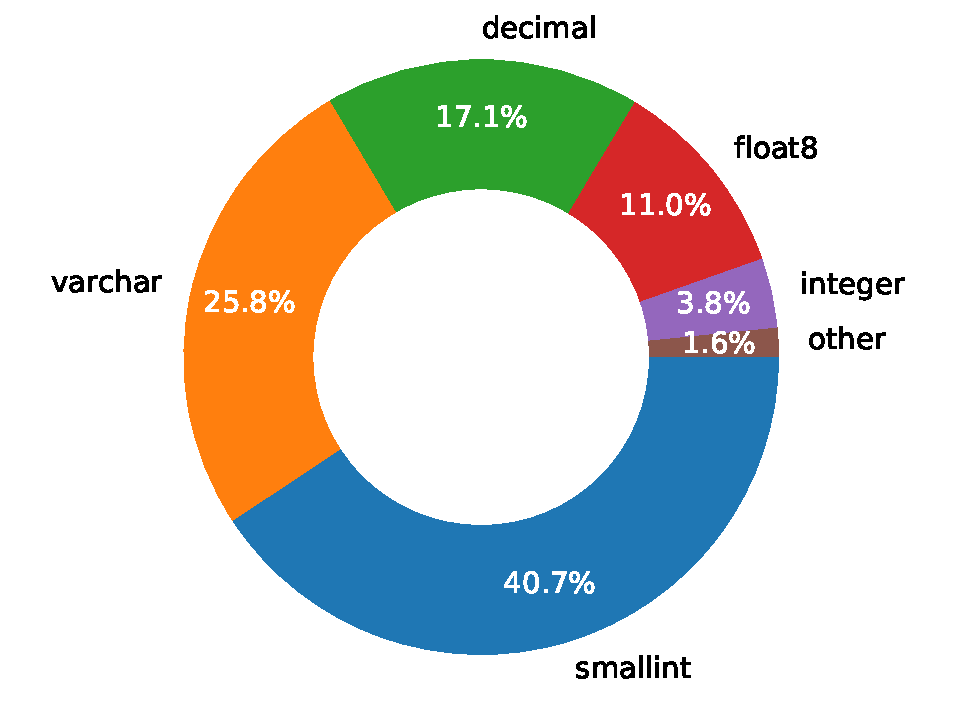
\includegraphics[width={1.0\linewidth}]{datatypes_total.pdf}
  \caption{Datatypes distribution}
  \label{fig:pbib:columnstats:datatypes}
\end{subfigure}
% \hspace{1em}
\begin{subfigure}[t]{0.55\linewidth}
  \centering
  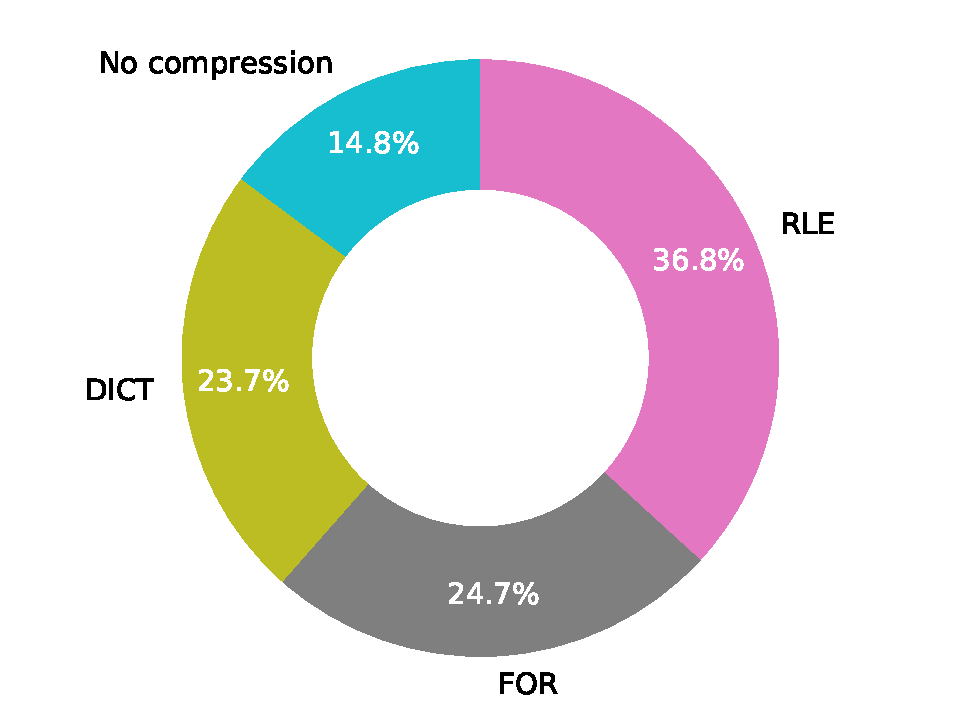
\includegraphics[width={1.0\linewidth}]{compression_methods_total.pdf}
  \caption{Compression potential}
  \label{fig:pbib:columnstats:estimators}
\end{subfigure}
}
\caption{Column statistics (percentage of columns)}
\label{fig:pbib:columnstats}
\end{figure}

Figure~\ref{fig:pbib:columnstats:datatypes} shows the distribution of datatypes across columns. The majority of the columns are numeric (73\%), followed by strings (25\%). The remaining columns are: \verb|DATE| (0.86\%), \verb|TIMESTAMP| (0.41\%), \verb|BIGINT| (0.17\%), \verb|BOOLEAN| (0.1\%), \verb|TIME| (0.05\%).

Given the focus of this thesis, we are interested in how suitable is the data for compression. We evaluated the potential of each column for compression with existing lightweight schemes: Run Length Encoding (RLE), Frame of Reference (FOR), Dictionary encoding (DICT). The evaluation was performed using the compression estimators defined in \ref{sub:estimators}~\nameref{sub:estimators}, following the methodology presented in \ref{fig:eval:methodology:estimatorbaseline}~\nameref{fig:eval:methodology:estimatorbaseline}. In short, we estimated the size of each column as compressed with RLE, FOR, DICT and uncompressed---based on a sample---and marked the column as a candidate for the method that gave the smallest size. The results are presented in Figure~\ref{fig:pbib:columnstats:estimators}. 85\% of the columns are good candidates for compression with lightweight schemes, while only 15\% of the columns are better left uncompressed. We applied DICT for \verb|VARCHAR| columns and RLE and FOR for \verb|numeric| columns. Most of the numeric columns are good candidates for RLE and FOR and the vast majority of \verb|VARCHAR| columns are dictionary compressible. The purpose of this analysis was to estimate the compression potential of the datasets in the benchmark. A more thorough analysis showing compression ratios and sizes is performed in \ref{sec:eval:resultsdiscussion}~\nameref{sec:eval:resultsdiscussion}.

\begin{figure}[h]
\centering
\makebox[\textwidth][c]{
\begin{subfigure}[t]{0.359\linewidth}
  \centering
  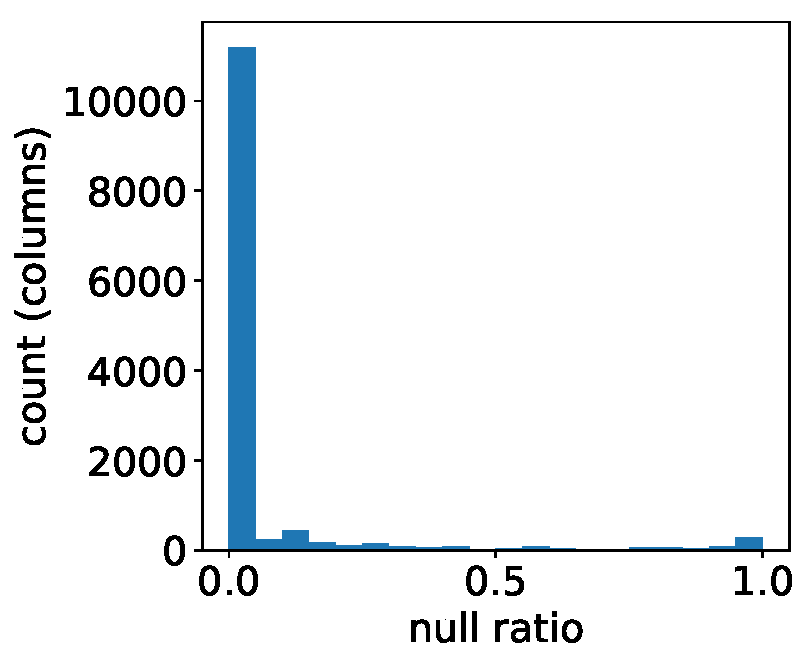
\includegraphics[width={1.0\linewidth}]{null_ratio.pdf}
  \caption{Null ratio}
  \label{fig:pbib:datastats:nulls}
\end{subfigure}
% \hspace{1em}
\begin{subfigure}[t]{0.35\linewidth}
  \centering
  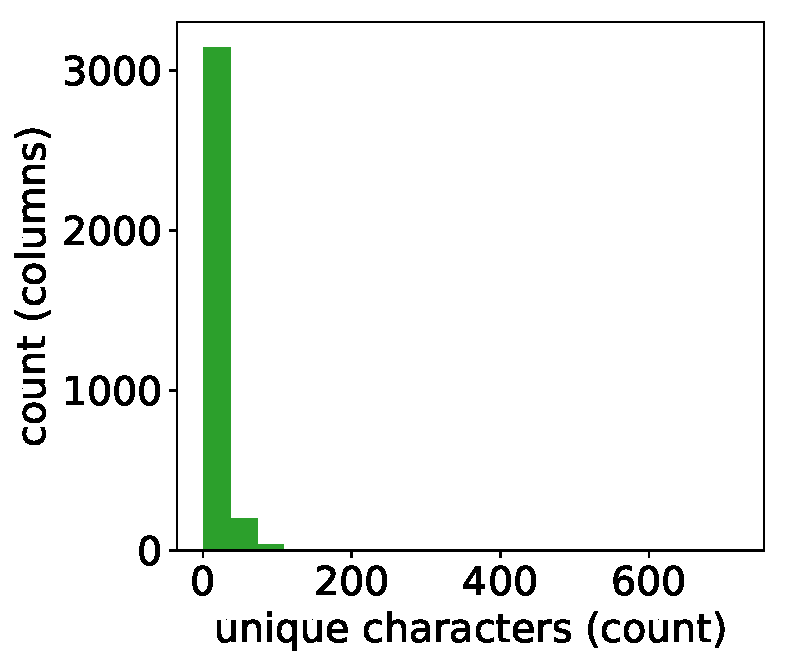
\includegraphics[width={1.0\linewidth}]{unique_chars.pdf}
  \caption{Unique characters}
  \label{fig:pbib:datastats:uniquechars}
\end{subfigure}
% \hspace{1em}
\begin{subfigure}[t]{0.359\linewidth}
  \centering
  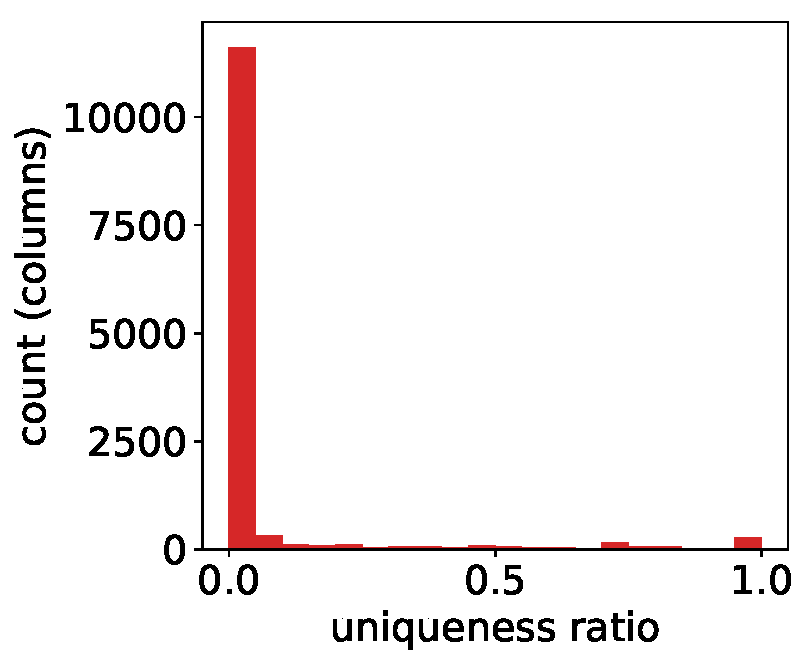
\includegraphics[width={1.0\linewidth}]{uniqueness_ratio.pdf}
  \caption{Uniqueness ratio}
  \label{fig:pbib:datastats:uniquenessratio}
\end{subfigure}
}
\caption{Data characterisation}
\label{fig:pbib:datastats}
\end{figure}

Figure~\ref{fig:pbib:datastats} shows metrics extracted with the \verb|statdump| command after loading the data into VectorWise \cite{zukowski2012vectorwise}. The percentage of null values is low for most of the columns. Figure~\ref{fig:pbib:datastats:uniquechars} shows the number of unique characters per column---for \verb|VARCHAR| columns: almost all of them have less than 100 unique characters. Only 8 columns have more than 255 unique characters and they contain social media content: posts or comments with hashtags and emoticons. Figure~\ref{fig:pbib:datastats:uniquenessratio} shows the uniqueness ratio of all the columns, irrespective of their datatype. The uniqueness of a column is computed as the number of unique values divided by the total number of values: \(\frac{unique_{count}}{total_{count}}\). Note that these metrics were computed based on the entire data and not based on a sample, therefore they are accurate. We notice how almost all of the columns have a very low uniqueness, indicating a high degree of repetition. This property makes the data suitable for compression and confirms the compression estimation results.
% \newline
% \newline

\subsection{Manual analysis}
So far we showed a general characterisation of the benchmark, mostly from a statistical point of view. In order to better understand the properties of real data and to gain more insight about it, we manually searched for patterns---common ways that users represent the data---with the purpose of finding opportunities for more compact representations. Below is a list of our findings:

\begin{itemize}
    % \item unstructured text
    % \item social media content---e.g. usernames, personal \& contact details, posts, comments, hashtags, emoticons
    % \item extended character set---UTF-8 characters from different languages, emoticons, etc.

    \item empty/missing values that are not nulls---e.g. empty quotes, whitespace characters;\\ examples:
    Eixo\_1\footnotemark: comunidade\_quilombola, unidade\_demandante
    
    \footnotetext{\url{https://github.com/cwida/public_bi_benchmark/blob/master/benchmark/Eixo/samples/Eixo\_1.sample.csv}}
    
    \item leading/trailing whitespace, some with the purpose of ensuring a common length of the values on \verb|VARCHAR| columns;\\ examples:
    CommonGovernment\_1\footnotemark: contract\_num, primary\_contract\_piid
    
    \item numbers and dates stored as strings in \verb|VARCHAR| columns;\\ examples:
    CommonGovernment\_1\footnotemark[\value{footnote}]: contract\_signeddate, agency\_code
    
    \item strings with fixed structure composed of substrings from different distributions---e.g. emails, urls, strings starting with a constant and ending in a number;\\ examples:
    CommonGovernment\_1\footnotemark[\value{footnote}]: co\_name, contract\_num
    
    \item correlations between columns---mostly as categorical variables, but also numeric correlations; special cases: identical columns;\\ examples:
    CommonGovernment\_1\footnotemark[\value{footnote}]: short\_name, ag\_name, description
    
    \footnotetext{\url{https://github.com/cwida/public_bi_benchmark/blob/master/benchmark/CommonGovernment/samples/CommonGovernment_1.sample.csv}}
\end{itemize}

All of these patterns are inefficient representations of the information, in terms of data storage. Some of them could have been avoided by the user (e.g. choosing the proper datatype for numeric values), while others are determined by the nature of the data itself. These patterns represent compression opportunities that cannot be exploited through existing compression schemes.
% \newline
% \newline
\subsection{Conclusion}
The conclusion that we can draw from the analysis we performed on the Public BI benchmark is that real data is redundant and represented in inefficient ways. It is already suitable for compression with existing lightweight methods, but it has a considerable untapped compression potential that could be exploited if the data had a different representation.

\iffalse
- scatter plot with skewness and kurtosis on distribution types background (see link from Benno) (Min/Max; Outliers characterisation; standard deviation; check if normal distribution; (in terms of distribution of numbers, dates, length of strings, character sets used, etc); metrics: range & standard deviation, mean (big skew = large range & big stdev), measures of spread = range and stdev)
\fi

% ---------------------------------------------------------------------------
% ----------------------- end of thesis sub-document ------------------------
% ---------------------------------------------------------------------------

% this file is called up by thesis.tex
% content in this file will be fed into the main document

\chapter{Compression language} % top level followed by section, subsection


% ----------------------- paths to graphics ------------------------



% ----------------------- contents from here ------------------------
% 

\section{Operators}
\label{sec:operators}


% ----------------------- paths to graphics ------------------------



% ----------------------- contents from here ------------------------
% 

% \subsection{}




% ---------------------------------------------------------------------------
% ----------------------- end of thesis sub-document ------------------------
% ---------------------------------------------------------------------------

\section{Expression tree}
\label{sec:exprtree}


% ----------------------- paths to graphics ------------------------



% ----------------------- contents from here ------------------------
% 

\subsection{Expression node}
\label{subsec:exprnode}




% ---------------------------------------------------------------------------
% ----------------------- end of thesis sub-document ------------------------
% ---------------------------------------------------------------------------

\section{Exception handling}


% ----------------------- paths to graphics ------------------------



% ----------------------- contents from here ------------------------
% 

% \subsection{}




% ---------------------------------------------------------------------------
% ----------------------- end of thesis sub-document ------------------------
% ---------------------------------------------------------------------------



% ---------------------------------------------------------------------------
% ----------------------- end of thesis sub-document ------------------------
% ---------------------------------------------------------------------------

% this file is called up by thesis.tex
% content in this file will be fed into the main document

\chapter{Automatic compression learning}
\label{ch:automaticlearning}


% ----------------------- paths to graphics ------------------------



% ----------------------- contents from here ------------------------
% 

This chapter presents our approach for automatically learning the best representation of a set of columns. We divided this problem into 2 smaller subproblems: 1) automatically identifying \textit{whitebox} representation opportunities in data; 2) automatically building a compression tree that minimizes the physical size of the data. They are described in the following sections.

\section{Pattern detection}
\label{sec:pd}


% ----------------------- paths to graphics ------------------------



% ----------------------- contents from here ------------------------
% 

TODO-1: brief description of pattern detection

\subsection{Generic pattern detector}
\label{subsec:genericpd}


% ----------------------- paths to graphics ------------------------



% ----------------------- contents from here ------------------------
% 

The purpose of a generic pattern detector is to serve as an interface in the pattern detection and compression learning processes. Given a sample of data and its schema, an instance of a generic pattern detector searches for the presence of the pattern it is specialized in.  For each column that matches the pattern, it outputs metrics and metadata that will be further used in the learning phase and during compression. This generic design allows new pattern detectors to be easily tested and integrated into the system without modifying other parts of it (e.g. the learning or compression processes). This section presents the characteristics of the generic pattern detector interface, while specialized implementations of it are described in the next sections.

The pattern detection process works in 3 phases: Phase-1: \textit{initialization}---initializes the pattern detector and creates the data structures that will be used in the next phases; Phase-2: \textit{scanning}---scans the sample of data and gathers information and metrics about values in the sample. Phase-3: \textit{evaluation}---aggregates the information gathered in the \textit{scanning} phase and produces an evaluation result.

\textbf{Parameters.} A pattern detector takes as input the following parameters:\\
a) \textit{columns}: id, name and datatype for each column\\
b) \textit{compression tree}: the compression tree built so far. Used in the \textit{select\_column} method\\
c) \textit{detection log}: history of the pattern detection process. Contains information about which pattern detectors were evaluated on each column and what was the result. Used in the \textit{select\_column} method.\\
Although most pattern detectors work on individual columns, some may work on multiple columns (e.g. \nameref{subsec:pd:columncorrelation}). For this reason we designed the generic pattern detector to search for patterns at the table level instead of individual columns.

\textbf{Methods.} A pattern detector must implement the following methods:\\
a) \textit{select\_column}: called in the \textit{initialization} phase---determines whether a given column will be processed by the pattern detector. The decision process is based on: 1) data type (e.g. string-specific patterns do not apply to numeric columns); 2) path in the compression tree that led to the creation of the column (e.g. \nameref{subsec:pd:columncorrelation} only applies to columns that are output of a \nameref{subsec:pd:dict} compression node); 3) history of the pattern detection process (e.g. do not evaluate a pattern detector on a column if it was already evaluated in a previous step). Column selection rules are listed in the section of each pattern detector.\\
b) \textit{feed\_tuple}: repeatedly called in the \textit{scanning} phase---processes a tuple. Data is fed to the pattern detector one tuple at a time. This method extracts information from the tuple that will be later used in the \textit{evaluate} method.\\
c) \textit{evaluate}: called in the \textit{evaluation} phase---aggregates the information extracted from the tuples fed so far and outputs the outcome of applying the pattern to the columns. See output details below.

\textbf{Output.} The result of evaluating a pattern detector on a sample of data is a list of \textit{(expression node, evaluation result)} tuples.\\
a) \textit{expression node}: describes how one or more \textit{input columns} are transformed into one or more \textit{output columns} by applying an \textit{operator} (see detailed description in \ref{ch:exprlang}~\nameref{ch:exprlang}). An important part here is the operator metadata that will be used to evaluate the \textit{expression node} in the (de)compression process (e.g. the operator metadata for the \nameref{subsec:pd:dict} pattern detector is the dictionary/map object).\\
b) \textit{evaluation result}: contains information used in the learning process and describes how well the \textit{input columns} of the \textit{expression node} match the pattern. It contains the following information: 1) \textit{coverage} (percentage of rows that the pattern applies to; i.e. \(1 - exception\_ratio\)); 2) \textit{row\_mask} (bitmap indicating the rows that the pattern applies to); 3) other pattern-specific evaluation results (e.g. correlation coefficient for column correlation).

Each \textit{(expression node, evaluation result)} tuple represents a possibility of applying the pattern on a subset of the columns. The same column may be present in multiple tuples since there may be more than one option of applying the pattern to it (e.g. the \nameref{subsec:pd:charsetsplit} pattern detector can split a column in 2 ways, because there are 2 dominant character set patterns on the column; see \ref{subsec:pd:charsetsplit}~\nameref{subsec:pd:charsetsplit} for more details). The \textit{row\_masks} for such a column may either be mutually exclusive or partially overlap. A pattern detector only outputs results for columns that match the pattern and are likely to produce good results in the compression process according to a pattern-specific estimator (e.g. \nameref{subsec:pd:dict} pattern detector only outputs tuples for columns that are dictionary compressible; see \ref{subsec:pd:dict}~\nameref{subsec:pd:dict} for more details).

\textbf{Operators.} Each pattern detector provides a \textit{compression operator} and a \textit{decompression operator}. They are used in the compression and respectively decompression phase to evaluate the nodes in the expression trees. The generic operator is described in \ref{ch:exprlang}~\nameref{ch:exprlang} while the pattern-specific implementations can be found in the corresponding section of each pattern detector.

% TODO-1: image describing the input and output of the generic pattern detector

% ---------------------------------------------------------------------------
% ----------------------- end of thesis sub-document ------------------------
% ---------------------------------------------------------------------------

\subsection{Constant}
\label{subsec:pd:constant}

\begin{verbatim}
TODO
\end{verbatim}

\subsection{Dictionary}
\label{subsec:pd:dict}

\begin{verbatim}
TODO
\end{verbatim}

\subsection{Numeric strings}
\label{subsec:pd:numericstrings}

\begin{verbatim}
TODO
\end{verbatim}

\subsection{Character set split}
\label{subsec:pd:charsetsplit}

\begin{verbatim}
TODO
\end{verbatim}

\subsection{n-gram frequency split}
\label{subsec:pd:ngramfreqsplit}

\begin{verbatim}
TODO
\end{verbatim}

\subsection{Column correlation}
\label{subsec:pd:columncorrelation}

\begin{verbatim}
TODO
\end{verbatim}

% ---------------------------------------------------------------------------
% ----------------------- end of thesis sub-document ------------------------
% ---------------------------------------------------------------------------

\section{Learning process}


% ----------------------- paths to graphics ------------------------



% ----------------------- contents from here ------------------------
% 

TODO-1: brief description and diagram of a compression learning algorithm

\subsection{Optimization problem}
\label{subsec:learningprocess:optimizationproblem}


% ----------------------- paths to graphics ------------------------



% ----------------------- contents from here ------------------------
% 

We can define the learning process as follows: given a sample from a dataset, its schema and a set of pattern detectors as input, output a compression tree that, when applied to the dataset, produces a compressed representation of it of minimum disk size.

The schema is a list of columns and their data types. The pattern detectors are implementations of the \nameref{subsec:genericpd}---receives the columns as input, evaluates the sample and returns a list of \textit{(expression node, evaluation result)} tuples. Adding an \textit{expression node} to the compression tree means: 1) altering the schema by deleting existing columns and creating new ones; 2) altering the sample by applying the \textit{compression operator} to the input columns and generating new data. The learning process can go on by recursively feeding the new schema and sample data to the pattern detectors, resulting in new \textit{(expression node, evaluation result)} tuples. This recursive process stops when no pattern detector outputs any result anymore---no pattern matches on the current schema and data.

Choosing to add or not an \textit{expression node} to the compression tree generates a new solution. This leads to a total number of \(2^n\) possible solutions (different compression trees), where \(n\) is the total number of \textit{expression nodes} generated by the recursive process (\(n\) binary decisions: \(1\) means adding a node and \(0\) not adding it). The total number of \textit{expression nodes} (\(n\)) depends on how well pattern detectors match on the initial columns and the newly generated ones. This is entirely dependent on the characteristics of the data and the patterns that were evaluated on it. In the worst case, all pattern detectors will match on any column, leading to the following expression for \(n\):
\begin{equation}
\label{eq:optimizationproblem:n}
    n = c_{in} \times (p \times \mathit{avg}(n_{p}) \times b) ^ h
\end{equation}
\begin{equation}
\label{eq:optimizationproblem:b}
    b = \mathit{avg}(c_{out})
\end{equation}
where:
\begin{itemize}
    \item[] \(n\) = total number of expression nodes
    \item[] \(c_{in}\) = number of input columns
    \item[] \(p\) = number of pattern detectors
    \item[] \(n_{p}\) = number of expression nodes returned by a pattern detector
    \item[] \(b\) = branching factor of the compression tree
    \item[] \(h\) = height of the compression tree
    \item[] \(c_{out}\) = number of output columns of an expression node
\end{itemize}

The score of each solution is given by the size of the compressed data that resulted after applying the compression tree to the dataset. The goal of the learning process is to choose the one that gives the smallest size.

The computational effort needed for each individual \textit{expression node} consists of: 1) applying the compression operator on its input columns to generate the new data (feeding each tuple in the sample data to the operator); 2) evaluating the pattern detectors on all the new columns (feeding each tuple in the sample data to each pattern detector). Moreover, some pattern detectors may need to evaluate combinations of columns instead of individual columns, which requires all the existing columns to be reevaluated for every newly generated column (e.g. \nameref{subsec:pd:columncorrelation} evaluates all pairs of 2 columns to determine the correlation coefficient between them).

\iffalse
TODO:
better formalize problem
https://en.wikipedia.org/wiki/Optimization\_problem
\fi

% ---------------------------------------------------------------------------
% ----------------------- end of thesis sub-document ------------------------
% ---------------------------------------------------------------------------

\subsection{Cost model: compression estimators}
\label{sub:estimators}

% ----------------------- paths to graphics ------------------------



% ----------------------- contents from here ------------------------
% 

The compression learning process is an optimization problem (\ref{subsec:learningprocess:optimizationproblem}) for finding the best compression tree in terms of disk size of the resulting physical columns. Solving the optimization problem requires a way to compare its solutions, i.e. estimating the final size of the compressed data. For this purpose we created a cost model which relies on leaf compression schemes size estimators (DICT, RLE, FOR, no compression) to predict the size of a column if compressed with these methods.

\textbf{Methodology}. The score of a solution (compression tree) is computed through the following methodology: 1) represent the sample data according to the compression nodes; 2) for each column of the new representation, estimate its size if it were compressed with: DICT, RLE, FOR or not compressed at all; 3) choose the smallest size among those. The result of this process is the smallest size of the new data representation if it were compressed with leaf compression schemes.

\textbf{System assumptions}. The size on disk of a compressed column depends on: 1) implementation of the compression method; 2) characteristics of the underlying database system. The former is described in the next sections as part of the estimator implementations. For the latter we defined some assumptions of the underlying system as follows:\\
a) \textit{data types}: strings are stored with null terminator, therefore their size is given by the number of characters + 1. For all other data types we consider the sizes used by Ingres Vectorwise \cite{zukowski2012vectorwise,actianingres}. \\
b) \textit{null handling}: we consider the same approach  used by Vectorwise \cite{zukowski2012vectorwise}: do not store null values, instead, keep track of their positions using a bitmap. This results in 1 additional bit for every attribute (for nullable columns).\\
c) \textit{exception handling}: we consider a whitebox approach: for each logical column store exceptions on a separate physical nullable column. The exception column has the same datatype as the logical column.

An additional assumption that we make about the underlying system is that it supports block-level compression, i.e. every block of data is compressed independently. This allows different compression schemes to be used on the same column, enabling the possibility to exploit local data characteristics.

\subsubsection{Generic compression estimator}
\label{subsub:estimator:generic}
A compression estimator takes as input a column and two samples of data (\textit{train} and \textit{test} sample) and outputs the estimated size of the compressed column. The result can be either the size of the compressed sample or the size extrapolated to the total size of the block or column. The latter requires an additional parameter specifying the total number of rows in the full data.

The estimated size has 4 components (exemplified for Dictionary encoding):\\
1) \(size_{metadata}\): size of the metadata (the dictionary itself)\\
2) \(size_{data}\): size of the compressed data (the dictionary ids)\\
3) \(size_{ex}\): size of the exceptions  (the values that are not in the dictionary)\\
4) \(size_{null}\): size required to keep track of the null values. Since exceptions are stored on a separate nullable column, the \textit{nulls} size is implicitly increased.

The final estimated size of the test sample is the sum of the 4 components:
\begin{equation}
\label{eq:estimators:sizesample}
size_{sample} = size_{metadata} + size_{data} + size_{ex} + size_{null}
\end{equation}

This result gives the size of the \textit{test} sample only. It can be extrapolated to the full size of the block or entire column as follows:
\begin{equation}
\label{eq:estimators:sizefinal}
size_{full} = size_{sample} \times \frac{count_{full}}{count_{sample}}
\end{equation}
where:
\begin{itemize}
    \item[] \(count_{sample}\) = total number of values in the test sample
    \item[] \(count_{full}\) = total number of values in the full block or column
\end{itemize}

The size estimation process works in two phases:\\
1) \textit{training}: the estimator analyzes the \textit{train} sample and generates the metadata needed for compression (e.g. \nameref{subsub:estimator:dict} generates the dictionary, \nameref{subsub:estimator:for} determines the reference value and the number of bits needed to store the differences).\\
2) \textit{testing}: the estimator simulates the compression of the \textit{test} sample using the metadata resulted from the \emph{training} phase and outputs an estimated size.

The two-phase estimation process is used to avoid overly-optimistic results: metadata generated based on the \emph{train} sample is perfectly optimized for that sample (e.g. in FOR all differences will fit in the number of bits chosen to represent them). Depending on the implementation of each compression estimator, this would lead to a reduced number of exceptions or even no exceptions at all. Therefore, the \textit{test} sample is used to provide new data for size estimation. It produces exceptions and more realistic results. This approach simulates the compression process of real database systems, where the compression metadata is created based on a sample and then applied on a full block of data or even on the entire column.

The next sections describes 4 compression estimators used in the learning process. All computed sizes will be in bytes.


% ------- no compression ------- % 

\subsubsection{No compression estimator}
\label{subsub:estimator:nocompression}

The \nameref{subsub:estimator:nocompression} predicts the size of the input column stored without compression. The \textit{training} phase is not relevant since it does not generate any compression metadata. The estimation is performed in the \textit{testing} phase, based on the size on disk of the column data type. The size components are computed as follows:

\(size_{metadata}\) is 0, since there is no compression metadata

\(size_{ex}\) is 0, since there are no exceptions

\(size_{null}\) is 1 bit for every value in the sample: 
\begin{equation}
\label{eq:estimators:nocompression:sizenull}
size_{null} = \frac{count_{sample}}{8}
\end{equation}
where:
\begin{itemize}
    \item[] \(count_{sample}\) = total number of values in the test sample
\end{itemize}

\(size_{data}\) is given by the total size of the non-null values in the sample. It depends on the data type of the column as follows:
\begin{equation}
\label{eq:estimators:nocompression:sizedata}
size_{data} = 
\left\{
\begin{array}{ll}
    \sum_{v \neq \mathit{null}} \mathit{len}(v) + 1 & \mbox{if } \mathit{datatype} = \verb|VARCHAR|\\
    count_{notnull} \times size_{datatype} & \mbox{else}
\end{array}
\right.
% \frac{count_{sample}}{8}
\end{equation}
where:
\begin{itemize}
    \item[] \(count_{notnull}\) = total number of non-null values in the test sample
    \item[] \(size_{datatype}\) = size on disk of the column data type
\end{itemize}


% ------- dictionary ------- % 

\subsubsection{Dictionary estimator}
\label{subsub:estimator:dict}

The \nameref{subsub:estimator:dict} predicts the size of the input column as compressed with Dictionary encoding. Besides the two samples, it receives an additional parameter: \(size_{max}\)---maximum size of the dictionary (in bytes). It only applies to \verb|VARCHAR| columns and therefore the exception column will also be \verb|VARCHAR|.

The \nameref{subsub:estimator:dict} is similar to the \nameref{subsec:pd:dict} pattern detector defined in \ref{subsec:pd:dict}. It builds the dictionary and handles exceptions in the same way. Optimizing the dictionary based on a maximum size (in bytes) also works for the estimator, since we use it to compare different ways of compressing a column and the dominant factor here is the nature of the data, not the optimization of the compression scheme. 

% Dictionary encoding only produces good results on columns that have a small number of unique values. However, it is hard to reliably quantify this property when analyzing only a sample of the data. Moreover, the distribution of unique values may be skewed, with only a few values with high frequency and a long tail of low frequency values. For the purpose of our estimator, we addressed this issue by enforcing a maximum dictionary size and only keeping the most common values in the dictionary. This approach is also suitable if blocks of data are compressed independently: dictionaries need to be small as they are assigned per block. There are other (possibly better) ways of optimizing the dictionary values and size. However, they are out of the scope of our estimator, since we use it to compare different ways of compressing a column and the dominant factor here is the nature of the data, not the optimization of the compression scheme.

\textbf{Training phase.} The dictionary (metadata) is built during the \textit{training} in same way it is done for the \nameref{subsec:pd:dict} pattern detector (\ref{subsec:pd:dict}): Step-1: create the histogram of all the values in the \textit{train} sample. Step-2: select as many values from the histogram in decreasing order of their number of occurrences such that their total size is lower or equal to the maximum size of the dictionary (\(size_{max}\)). The dictionary is stored as an array containing the selected values. The indices in the array represent the dictionary ids used to encode the values.

\(size_{metadata}\) is given by the total size of the values in the dictionary. Additionally, the number of bits required to store a dictionary id is computed as follows:
\begin{equation}
\label{eq:estimators:dict:bitsid}
bits_{id} = \lceil \log_2 (count_{entries}) \rceil
\end{equation}
where:
\begin{itemize}
    \item[] \(count_{entries}\) = number of values in the dictionary
\end{itemize}

\textbf{Testing phase}. The \textit{testing} phase estimates the size of the compressed column by going through each value in the \textit{test} sample and checking if it is present in the dictionary. The following variables are updated in this process: 1) \(count_{valid}\): number of values that are found in the dictionary; 2) \(size_{ex}\): size of the exceptions (values that are not found in the dictionary).

\(size_{data}\) is computed as follows:
\begin{equation}
\label{eq:estimators:dict:sizedata}
size_{data} = \frac{count_{valid} \times bits_{id}}{8}
\end{equation}

\(size_{ex}\) is computed by summing the size of all exceptions.

\(size_{null}\) is determined by the number of resulting physical columns: one for compressed data (dictionary ids) and one for exceptions:
\begin{equation}
\label{eq:estimators:dict:sizenull}
size_{null} = \frac{2 \times count_{sample}}{8}
\end{equation}
where:
\begin{itemize}
    \item[] \(count_{sample}\) = total number of values in the test sample
\end{itemize}


% ------- run length encoding ------- % 

\subsubsection{Run Length Encoding estimator}
\label{subsub:estimator:rle}

The \nameref{subsub:estimator:rle} predicts the size of the input column as compressed with RLE. Even though RLE can be applied to any data type, we limited the scope of our estimator to numeric columns. The other data types are either compressed with Dictionary encoding (\verb|VARCHAR|) or are very rare in the Public BI benchmark and do not present compression opportunities. We use the following terminology:\\
1) \textit{run} value = a data value that is repeated on consecutive rows.\\
2) \textit{length} value = the number of consecutive occurrences of a \textit{run} value

\textbf{Training phase.} RLE metadata is composed of: 1) the number of bits needed to represent the \textit{run} values (\(bits_{run}\)) and 2) the number of bits needed to represent the \textit{length} values (\(bits_{length}\)). These values are determined by scanning the \textit{train} sample and computing all the \textit{runs} and \textit{lengths}. \(bits_{run}\) is given by the \textit{run} value of maximum size and \(bits_{length}\) is given by the maximum \textit{length}. \(bits_{run}\) also depends on the column data type representation.

\(size_{metadata}\) is between 8 and 24 bytes---the size of 2 numbers: \(bits_{run}\) and \(bits_{length}\)---depending on the data types used to store them.

\textbf{Testing phase.} The \textit{testing} phase scans all the values in the \textit{test} sample and creates (\textit{run}, \textit{length}) pairs as follows: 1) if a \textit{run} value cannot be represented on \(bits_{run}\) bits: mark it as exception and skip it; 2) if a \textit{length} exceeds the maximum value that can be represented on \(bits_{length}\) bits: end the current run at this length and start a new run. The following variables are updated in this process: 1) \(count_{valid}\): the number of (\textit{run}, \textit{length}) pairs resulted from the scanning process; 2) \(count_{ex}\): the number of exceptions as defined above.

\(size_{data}\) and \(size_{ex}\) are computed as follows:
\begin{equation}
\label{eq:estimators:rle:sizedata}
size_{data} = \frac{count_{valid} \times (bits_{run} + bits_{length})}{8}
\end{equation}
\begin{equation}
\label{eq:estimators:rle:sizeex}
size_{ex} = count_{ex} \times size_{datatype}
\end{equation}
where:
\begin{itemize}
    \item[] \(size_{datatype}\) = size on disk of the column data type
\end{itemize}

\(size_{null}\) depends on the number of physical columns---one compressed data column (\textit{run} and \textit{length} are stored together) and one exception column---the same as in the case of \nameref{subsub:estimator:dict} (Equation \ref{eq:estimators:dict:sizenull}).


% ------- frame of reference ------- % 

\subsubsection{Frame of Reference estimator}
\label{subsub:estimator:for}

The \nameref{subsub:estimator:for} predicts the size of the input column as compressed with FOR. It only applies to numeric columns.

\textbf{Training phase.} FOR metadata is composed of: 1) the \textit{reference} value and 2) the number of bits needed to store the differences (\(bits_{\mathit{diff}}\)). In our implementation we chose the \textit{reference} to be the smallest value in the \textit{train} sample. \(bits_{\mathit{diff}}\) is given by the maximum difference size, which depends on the data type representation.

\(size_{metadata}\) is between 8 and 24 bytes---the size of the reference and the size of \(bits_{\mathit{diff}}\)---depending on the data types used to store them.

\textbf{Testing phase.} The testing phase computes all the differences between the values in the \textit{test} sample and the \textit{reference} and filters the ones that can be represented on \(bits_{\mathit{diff}}\) bits. The following variables are updated in this process: 1) \(count_{valid}\): the number of differences that fit in \(bits_{\mathit{diff}}\); 2) \(count_{ex}\): the number of exceptions (values that give differences larger than \(bits_{\mathit{diff}}\)).

\(size_{data}\) is computed as follows:
\begin{equation}
\label{eq:estimators:for:sizedata}
size_{data} = \frac{count_{valid} \times bits_{\mathit{diff}}}{8}
\end{equation}

\(size_{ex}\) is the same as in the case of \nameref{subsub:estimator:rle} (Equation \ref{eq:estimators:rle:sizeex}).

\(size_{null}\) depends on the number of physical columns---one compressed data column (differences) and one exception column---the same as in the case of \nameref{subsub:estimator:rle} and \nameref{subsub:estimator:dict} (Equation \ref{eq:estimators:dict:sizenull}).

% ---------------------------------------------------------------------------
% ----------------------- end of thesis sub-document ------------------------
% ---------------------------------------------------------------------------

\subsection{Recursive exhaustive learning}
\label{sub:learning:recursiveexhaustive}


% ----------------------- paths to graphics ------------------------



% ----------------------- contents from here ------------------------
% 

This section presents an exhaustive recursive algorithm for compression learning. It uses the compression estimators (\(E\)) as a cost model (\ref{sub:estimators}~\nameref{sub:estimators}) and the pattern detectors (\(P\)) defined in \ref{sec:pd}~\nameref{sec:pd}. The algorithm takes as input a column (\(c_{in}\)) and outputs the best compression tree (\(T_{out}\)) with respect to the compression estimators: the one that produces the smallest representation of the column when used to compress it. The algorithm is recursive and takes a depth-first approach. For this reason, it is not suitable for pattern detectors that work with more than one column (e.g. \nameref{subsec:pd:columncorrelation}).

In addition to the input column \(c_{in}\), the recursive function receives a compression tree \(T_{in}\) (initially empty) and an optional max height parameter \(h_{max}\) (the maximum height of the compression tree). The compression tree \(T_{in}\) is the partial solution built in the recursive process so far. The role of the \(h_{max}\) parameter is to limit the dimension of the problem and avoid scenarios where the algorithm does not finish .

The algorithm tries all possibilities to compress the input column \(c_{in}\): 1) with leaf compression nodes (\(N_{leaf}\), e.g. RLE, FOR, DICT); 2) with internal (non-leaf) compression nodes (\(N_{internal}\), e.g. \nameref{subsec:pd:numericstrings}, \nameref{subsec:pd:charsetsplit}, etc.); 3) no compression. For each possibility it estimates the size of the resulting columns (\(c_{out}\)) in the following way: 1) for leaf compression nodes \(N_{leaf}\) and no compression the estimators \(E\) directly provide the size; 2) for non-leaf compression nodes \(N_{internal}\) the size is computed by recursively applying the same algorithm on the output columns \(c_{out}\) of the compression node \(N_{internal}\) and adding the resulted sizes together. The recursive call returns a new compression tree \(T_{c}\) for each output column of \(N_{internal}\). A special case is the DICT compression node, which will have 2 estimated sizes: 1) direct estimation from the \nameref{subsub:estimator:dict} \(E_{dict}\) as a leaf node; 2) recursive call estimation (other pattern detectors \(P\) can be applied on its output column, e.g. \nameref{subsec:pd:columncorrelation}).

Out of all the possibilities to compress \(c_{in}\), the one which gives the smallest size is chosen and \(T_{in}\) is updated with either the leaf compression node \(N_{leaf}\) or with the set of compression trees \(T_{c}\) resulted from the recursive call. The algorithm returns the updated compression tree \(T_{out}\).

The termination conditions of the recursive algorithm are: 1) all possibilities to compress \(c_{in}\) are leaf compression nodes (i.e. there is no \(N_{internal}\) to generate new output columns \(c_{out}\)); 2) the max height of the compression tree \(h_{max}\) is reached. Termination condition 1) occurs when no pattern detector \(P\) outputs any compression nodes \(N_{internal}\). A pattern detector \(P\) does not output any compression node \(N_{internal}\) when: 1) \(c_{in}\) is not compatible with the pattern (e.g. \nameref{subsec:pd:numericstrings} pattern detector only works on \verb|VARCHAR| columns; see \textit{select\_column} in \ref{sec:pd}~\nameref{sec:pd}); 2) the data in \(c_{in}\) does not match the pattern (e.g. a column with multiple values does not match the \nameref{subsec:pd:constant} pattern).

The algorithm is described in listings \ref{lst:learning:recursiveexhaustive:build_T} and \ref{lst:learning:recursiveexhaustive:apply_N}.

\begin{lstlisting}[language=Python,
label={lst:learning:recursiveexhaustive:naming},
caption={Naming conventions}]
c = column
T = compression tree
E = compression estimator
P = pattern detector
N = compression node
\end{lstlisting}

\begin{lstlisting}[language=Python,
label={lst:learning:recursiveexhaustive:build_T},
caption={build\_T (recursive exhaustive)}]
def build_T(c_in, T_in, P_list, E_list):
  sol_list = list()
  # estimator evaluation
  for E in E_list:
    size = E.evaluate(c_in)
    sol_list.append((size, T_in))
  # pattern detection 
  N_list = list()
  for P in P_list:
    N_p_list = P.evaluate(c_in)
    N_list.extend(N_p_list)
  # recursive evaluation
  for N in N_list:
    (size, T_out) = apply_N(c_in, N, T_in, P_list, E_list)
    sol_list.append((size, T_out))
  # return best solution
  return min(sol_list, key=size)
\end{lstlisting}

\begin{lstlisting}[language=Python,
label={lst:learning:recursiveexhaustive:apply_N},
caption={apply\_N (recursive exhaustive)}]
def apply_N(c_in, N, T_in, P_list, E_list):
  T_out = copy(T_in)
  T_out.update(N)
  # recursive call for all output columns
  sol_list = list()
  for c_out in N.c_out_list:
    (size_c, T_c) = build_T(c_out, T_out, P_list, E_list)
    sol_list.append((size_c, T_c))
  # merge results
  size_out = 0
  for (size_c, T_c) in sol_list:
    size_out += size_c
    T_out = merge(T_out, T_c)
  # return merged result
  return (size_out, T_out)
\end{lstlisting}
\bigskip

The complexity of the algorithm can be described as follows:
\begin{equation}
\label{eq:learning:recursiveexhaustive:single}
    (p \times \mathit{avg}(n_{p}) \times b) ^ {h_{max}}
\end{equation}
where:
\begin{itemize}
    \item[] \(p\) = number of pattern detectors
    \item[] \(n_{p}\) = number of expression nodes returned by a pattern detector
    \item[] \(b\) = branching factor of the compression tree (as defined in Equation \ref{eq:optimizationproblem:b})
    \item[] \(h_{max}\) = maximum height of the compression tree
\end{itemize}
The height is bounded by the \(h_{max}\) parameter. Despite the high complexity, the size of the problem remains relatively small due to the high selectivity of the pattern detectors \(P\) (see \textit{select\_column} in \ref{sec:pd}~\nameref{sec:pd}). This is the complexity of learning the compression tree for a single column, while for multiple columns the complexity becomes:
\begin{equation}
\label{eq:learning:recursiveexhaustive:multi}
    c_{in} \times (p \times \mathit{avg}(n_{p}) \times b) ^ {h_{max}}
\end{equation}
where:
\begin{itemize}
    \item[] \(c_{in}\) = number of input columns
\end{itemize}

This complexity is significantly better than the complexity of the general optimization problem described in \ref{subsec:learningprocess:optimizationproblem} (\(2^n\), where \(n\) is the total number of expression nodes generated in the learning process, as described in Equation~\ref{eq:optimizationproblem:n}). The reason for this improvement is the single-column approach---not considering pattern detectors \(P\) that combine multiple columns. The solutions of a column \(c_{i}\) do not depend on the solutions of other columns \(c_{j}\) that are not on the path from \(c_{i}\) to its root input column \(c_{r}\). This is because a choice made for \(c_{j}\) does not influence the choices that can be made for \(c_{i}\).
This property allows a depth-first exploration of the solutions, significantly reducing the complexity.

However, there is a cost for not considering multi-column pattern detectors: the algorithm misses compression opportunities (e.g. one column represented as a function of another through \nameref{subsec:pd:columncorrelation}). It is exhaustive and yet cannot produce the best result. Section \ref{sub:learning:iterative}~\nameref{sub:learning:iterative} presents a greedy approach that considers multi-column patter detectors. Moreover, the \nameref{sub:learning:multistage} in section \ref{sub:learning:multistage} addresses this issue by chaining together multiple learning algorithms.

% ---------------------------------------------------------------------------
% ----------------------- end of thesis sub-document ------------------------
% ---------------------------------------------------------------------------

\subsection{Pattern selectors}
\label{sub:learning:selectors}

% ----------------------- paths to graphics ------------------------

\graphicspath{{5_automatic_learning/learning_process/images/}}

% ----------------------- contents from here ------------------------
% 

Section \ref{sub:learning:recursiveexhaustive} described an exhaustive learning algorithm based on compression estimators (\ref{sub:estimators}). A greedy learning algorithm based on \emph{pattern selectors} will be described in section \ref{sub:learning:iterative}. Pattern selectors are decision algorithms used to make greedy choices in the compression learning process. This section describes the general characteristics of a pattern selector and specialized instances of it.

\subsubsection{Generic pattern selector}
\label{subsubsec:ps:generic}

A generic pattern selector is an abstraction used in the learning process for selecting the \textit{expression nodes} that will be added to the compression tree. Given a list of \textit{(expression node, evaluation result)} tuples resulted in the pattern detection phase, it outputs a subset of the expression trees provided as input. This selection process is necessary as there are multiple ways of representing the same column. The generic pattern selector chooses the best \textit{expression nodes} according to a set of criteria. Different implementations of pattern selectors are described below.

% TODO-2: [?] image describing the input and output of the generic pattern selector; not necessary but may be added for completeness and for reuse in the learning algorithms diagrams

\subsubsection{Coverage pattern selector}
\label{subsubsec:ps:coverage}

The coverage pattern selector tries to maximize the coverage of each column (i.e. minimize the exception ratio). It has 2 operation modes: 1) \textit{single-pattern}: selects the \textit{expression node} with the highest coverage; 2) \textit{multi-pattern}: selects the best combination of \textit{expression nodes} that give the largest coverage when used together on the same column.

The values on a column usually fall in different, possibly overlapping, pattern types. It is rarely the case that one pattern perfectly fits to all the values in a column. In most cases there is either one dominant pattern and the rest of the values are just noise, or multiple patterns that together cover all the values on the column. An example could be a \verb|VARCHAR| column where half of the values are numbers and the other half are concatenations of a constant with numbers.

The \textit{single-pattern} operation mode will select only one expression node---the one with the highest coverage. The \textit{multi-pattern} operation mode will select multiple expression nodes, such that their combined coverage of the column is maximal. We defined 2 approaches for the \textit{multi-pattern} mode: 1) a Greedy algorithm that selects one expression node at a time---the one with the highest coverage---until the column is fully covered or there are no more expression nodes to choose from; 2) an exhaustive algorithm that tries every combination of expression nodes and outputs the one with the highest cumulative coverage. Both approaches can further take into account the following parameter: \(coverage_{min}\)---minimum coverage that determines whether a pattern is considered or not.

The combined coverage of 2 patterns \(p_{a}\) and \(p_{b}\) can be computed based on their \textit{row\_masks} \(\mathit{rm}_{a}\), \(\mathit{rm}_{b}\)---defined in \ref{subsec:genericpd}---through a bitwise \verb|OR| operation: \(\mathit{rm}_{combined} = \mathit{rm}_{a} | \mathit{rm}_{b}\). The number of bits of a \textit{row\_mask} is equal to the number of rows in the table: \(r\). The combined coverage is then computed as the number of \(1\) bits in \(\mathit{rm}_{combined}\) divided by \(r\).

The complexity of these algorithms depends on the number of patterns found on the column: \(p\). The \textit{single-pattern} operation mode and the Greedy algorithm for the \textit{multi-pattern} mode both have a linear complexity. The exhaustive algorithm has an exponential complexity, as it tries all combinations of patterns: for \(p = 10\) there are \(10^3\) bitwise \verb|OR| operations on \(r\)-bit numbers, while for \(p = 27\) this number grows to \(10^9\). Equation~\ref{eq:ps:coverage:exhaustive} shows the complexity of the exhaustive algorithm.
\begin{equation}
\label{eq:ps:coverage:exhaustive}
    \sum_{k=1}^{p} {p \choose k}
\end{equation}

We implemented a basic version of the exhaustive approach for the \textit{multi-pattern} mode. To avoid the exponential running time, we default to the \textit{single-pattern} mode if the number of patterns \(p\) is larger than 20. In practice, we never encountered more than 20 different patterns on the same column, therefore, the exhaustive approach is a suitable choice.

Both operation modes give similar results in terms of physical representation of the data, but the resulting expression trees have different shapes. The \textit{single-pattern} mode selects only one expression node, moving the other values on an exception column. If the learning algorithm supports recursive expression of exception columns, then the most dominant pattern in the exception column is further selected, resulting in a new expression node on a new level of the tree. This process creates deep expression trees. In contrast, the \textit{multi-pattern} mode adds all expression nodes on the same level of the tree, resulting in wider but shorter expression trees. The evaluation of expression trees resulted from \textit{multi-pattern} selection is described in \ref{sec:exprlang:compdecomp}~\nameref{sec:exprlang:compdecomp}.

\subsubsection{Priority pattern selector}
\label{subsubsec:ps:priority}

The purpose of this pattern selector is to choose the best expression node based on pattern priorities. In addition to the \textit{expression node} list, it also receives a set of priority classes for pattern detector types. Each priority class contains a list of pattern types (e.g. \nameref{subsec:pd:numericstrings}, \nameref{subsec:pd:charsetsplit}, etc.) and a pattern selector that will be used to select the patterns in the same class. The selection process works in the following way:\\
1) for each column, select only the \textit{expression nodes} with the highest priority---their associated pattern type has the highest priority according to the provided list;\\
2) further select these \textit{expression nodes} using the pattern selector provided for their priority class and output the result.

An example of an input priority set is shown in Table~\ref{tab:ps:priority:table1}.

\input{5_automatic_learning/learning_process/pattern_selection-table_1.tex}

Given a column \(c\) and the priority set in Table~\ref{tab:ps:priority:table1}, the \nameref{subsubsec:ps:priority} will proceed as follows. It will first search for a \nameref{subsec:pd:constant} expression node that has \(c\) as input. If found, \(c\) will be represented as a constant. Since the \nameref{subsec:pd:constant} pattern detector outputs only one result per column, there is no need for a pattern selector on the constant priority class---the only constant expression node will be chosen. If there is no constant expression node, the pattern selector will search for expression nodes in the next priority class: \nameref{subsec:pd:dict} and \nameref{subsec:pd:numericstrings}. Both pattern detectors output a single result per column, thus there is a maximum of 2 expression nodes to choose from. The \nameref{subsubsec:ps:coverage} will be used to choose between them. Finally, if no expression node was found yet, the selector moves to the last priority class. It searches for \nameref{subsec:pd:charsetsplit} expression nodes.
There can be multiple instances of the \nameref{subsec:pd:charsetsplit} pattern detector initialized with different parameters and each instance can output multiple results for the same column. The \nameref{subsubsec:ps:coverage} is used to choose the best combination of results such that the total coverage of the column is maximized.

\subsubsection{Correlation pattern selector}
\label{subsubsec:ps:correlation}

This pattern selector is specialized in \nameref{subsec:pd:columncorrelation} \textit{expression nodes}. The \nameref{subsec:pd:columncorrelation} pattern detector outputs all the correlations between the columns in the dataset, resulting in multiple possibilities of representing the same column as a function of other columns---multiple \textit{(source, target)} pairs with the same target column. The \nameref{subsubsec:ps:correlation} selects the \textit{expression nodes} such that every \textit{target} column is represented by a single \textit{source} column, while also trying to maximize the average correlation coefficient and avoid circular dependencies.

We can make the following observation: the column correlation as defined in \ref{subsec:pd:columncorrelation} is a transitive relation. We formalized this observation in Theorem~\ref{subsec:ps:corr:theorem1}.

\begin{theorem}
\label{subsec:ps:corr:theorem1}
Let \(c_{a}\), \(c_{b}\), \(c_{c}\) be three columns and let \(c_{a} \xrightarrow{m_{ab}} c_{b}\) be the correlation relation meaning: \(c_{a}\) determines \(c_{b}\) through a mapping \(m_{ab}\). If \(c_{a} \xrightarrow{m_{ab}} c_{b}\) and \(c_{b} \xrightarrow{m_{bc}} c_{c}\) then \(c_{a} \xrightarrow{m_{ac}} c_{c}\).
\end{theorem}
\begin{proof}
Let \((v_{a}, v_{b})\) be an entry in \(m_{ab}\)---meaning: value \(v_{a}\) on column \(c_{a}\) always corresponds to value \(v_{b}\) on column \(c_{b}\)---and let \((v_{b}, v_{c})\) be an entry in \(m_{bc}\). Then, value \(v_{a}\) on column \(c_{a}\) always corresponds to value \(v_{c}\) on column \(c_{c}\). Therefore, \(\exists\) \(m_{ac}\)---a mapping containing the entry \((v_{a}, v_{c})\)---and \(c_{a} \xrightarrow{m_{ac}} c_{c}\).
\end{proof}

We define the correlation graph as follows: directed graph with one or more connected components; nodes represent columns; \textit{(src, dst)} edges represent correlations: column \textit{dst} is determined by column \textit{src}. The weight of an edge is the correlation coefficient between \textit{src} and \textit{dst}. An example of a correlation graph is shown in Figure~\ref{fig:ps:columncorrelation:corrgraph1}. The red edges represent an optimal selection in terms of the metrics and conditions described in the following paragraphs. This figure shows a simple correlation graph, but in practice we encountered much complex graphs resulted from the learning process for tables with highly correlated data.

\begin{figure}[h]
  \centering
  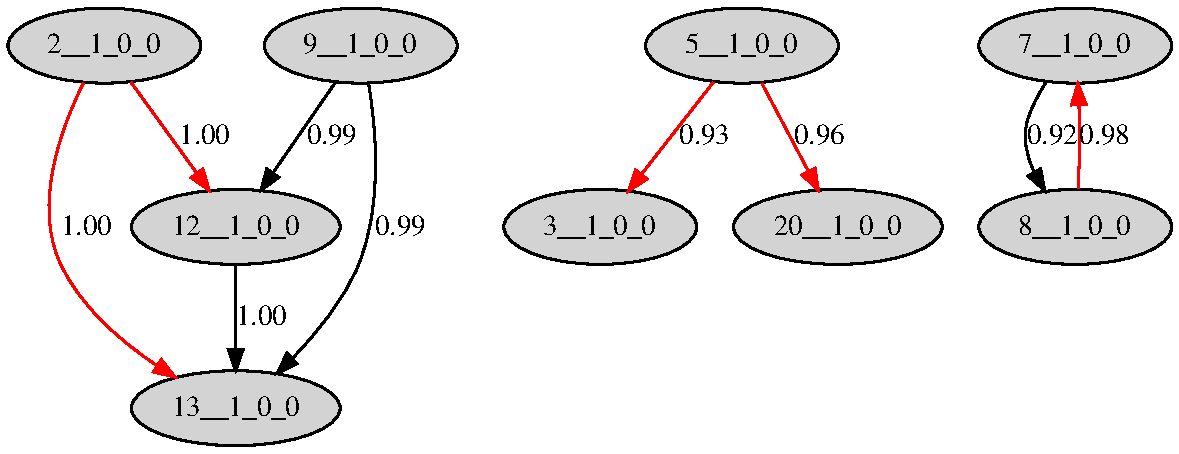
\includegraphics[width={0.9\linewidth}]{corr_graph_1.pdf}
  \caption{Correlation graph}
  \label{fig:ps:columncorrelation:corrgraph1}
\end{figure}

The main goal of the \nameref{subsubsec:ps:correlation} is to select a subset of the edges in the graph. We can define this process as the optimization problem of selecting a subset of edges in the correlation graph \(G\) such that the resulting subgraph \(G_{s}\) satisfies the following properties (in this order):
\begin{itemize}
    \item[\textit{P1}:] the indegree of any node is at most 1---a column should be determined by no more than 1 other column
    \item[\textit{P2:}] any path in \(G_{s}\) is of length 1---because of the transitivity property, for every path between nodes \(c_{a}\) and \(c_{b}\), there will also be a direct edge from \(c_{a}\) to \(c_{b}\)
    \item[\textit{P3}:] the number of nodes in \(G_{s}\) with indegree > 0 is maximal---the number of columns that are represented as functions of other columns is maximal
    \item[\textit{P4}:] the average weight of the edges is maximal---the edges with the highest correlation coefficient should be selected
\end{itemize}

We defined a Greedy algorithm for solving the correlation selection optimization problem. It builds the \(G_{s}\) graph by greedily selecting one edge at a time from \(G\). The edge is added to \(G_{s}\), \(G\) is updated and the process goes on until there are no more edges in \(G\). The algorithm is described in listings \ref{lst:ps:corr:selectcorr}, \ref{lst:ps:corr:nodescore}, \ref{lst:ps:corr:edgescore}.

\begin{lstlisting}[language=Python,
label={lst:ps:corr:selectcorr},
caption={select\_correlations}]
# G = correlation graph resulted from the correlation detection process
def select_correlations(G):
  G_s = <empty correlation graph>
  while G.edges is not empty:
    # select destination node
    dst = min(G.nodes, key=get_node_score)
    # select (_, dst) edge
    (src, dst, corr_coef) = min(dst.incoming_edges, key=get_edge_score)
    # update G_s
    G_s.add((src, dst, corr_coef))
    # update G
    G.remove(dst.incoming_edges)
    G.remove(dst.outgoing_edges)
    G.remove(dst)
    G.remove(src.incoming_edges)
  return G_s
\end{lstlisting}

\begin{lstlisting}[language=Python,
label={lst:ps:corr:nodescore},
caption={get\_node\_score}]
def get_node_score(node):
  indegree_src = min([src.indegree 
                     for (src, dst) in node.incoming_edges])
  return (node.outdegree, indegree_src, node.indegree)
\end{lstlisting}

\begin{lstlisting}[language=Python,
label={lst:ps:corr:edgescore},
caption={get\_edge\_score}]
def get_edge_score((src, dst, corr_coef)):
  return (src.indegree, -corr_coef, -src.out_degree)
\end{lstlisting}
\bigskip

Every iteration of the \textit{while} loop first selects the destination node of the candidate edge based on its score. The \textit{get\_node\_score} function prioritizes nodes with the minimum outdegree---ideally 0---such that the number of discarded edges as an effect of constraint \textit{P2} is minimized. The difference between nodes with the same outdegree is made by the minimum indegree of its parent nodes (source nodes of incoming edges)---for the same reason. Finally the difference is further made by the smallest indegree of the node itself, prioritizing columns with fewer options of being represented as functions of other columns. 

With the destination node fixed, the best edge is selected from its incoming edges. The \textit{get\_edge\_score} function prioritizes edges that have a minimum indegree---ideally 0---such that nodes at the start of correlation paths are selected. The difference between these nodes is further made based on the highest correlation coefficient and then by the highest outdegree.

The selected edge is added to \(G_{s}\) and \(G\) is updated such that constraints \textit{P1} and \textit{P2} are satisfied: the destination node, its incoming and outgoing edges and the incoming edges of the source node are removed. This process changes the degree of the nodes in \(G\) and impacts their scores.

The complexity of the algorithm, as described above, is given by the number of nodes in \(G\) and their average indegree: \(N^2 \times avg(indegree)\), where \(N\) is the number of nodes. Every iteration of the \textit{while} loop selects one node from \(G\) by computing the score of all nodes. The \textit{get\_node\_score} function loops through all incoming edges of the node. If the selection of the \(dst\) node is done with a priority queue the complexity is improved: \(N \times \log(N) \times avg(indegree)\).

An alternative approach would be to relax constraint \textit{P2} and allow paths of length higher than 1. Then apply a variation of the Dijkstra's shortest paths algorithm to shorten these paths with the goal of minimizing the complexity of the graph without affecting its average correlation coefficient. However, relaxing  \textit{P2} imposes a new constraint on \(G_{s}\): it should not contain any cycles. We leave this approach for future work.

% ---------------------------------------------------------------------------
% ----------------------- end of thesis sub-document ------------------------
% ---------------------------------------------------------------------------

\subsection{Iterative greedy learning}
\label{sub:learning:iterative}


% ----------------------- paths to graphics ------------------------



% ----------------------- contents from here ------------------------
% 

This section presents a greedy iterative algorithm for compression learning. It uses a pattern selector (\(S\)) to greedily choose how to compress columns (\ref{sub:learning:selectors}~\nameref{sub:learning:selectors}) and the pattern detectors (\(P\)) defined in \ref{sec:pd}~\nameref{sec:pd}. The algorithm takes a breadth-first approach, thus supporting pattern detectors \(P\) that work on multiple columns (e.g. \nameref{subsec:pd:columncorrelation}). It takes as input the list of input columns (\(c_{in}\)) and builds the compression tree one level at a time.

% https://en.wikipedia.org/wiki/Iterated_function
The algorithm builds the compression tree \(T\) in an iterative process. Let \textit{add\_level(\(T\))} be an iterated function which adds 0 or more expression nodes (\(N\)) on a new level in \(T\). This function is repeatedly applied to T in an iterative process. Each call of the function uses the updated version of \(T\) that it produced in the previous iteration. The iterative process converges to the final compression tree \(T_{out}\) once no more changes are made to \(T\) in an iteration.

The learning algorithm starts with \(P_{list}\) (a list of pattern detector instances), \(S\) (a pattern selector) and \(T\) (an empty compression tree, initialized with the list of input columns \(c_{in}\)). Recall that the compression tree is actually a graph with multiple connected components where each component is a directed acyclic graph with one or more root nodes (see \ref{sec:exprtree}~\nameref{sec:exprtree}). An additional parameter is \(it_{max}\), representing the maximum number of iterations. \(it_{max}\) also determines the maximum height of the compression tree (\(h_{max}\)), since every iteration adds a new level to \(T\).

The \textit{add\_level} function adds new compression nodes (\(N\)) to \(T\) by trying to further compress its leaf (output) columns \(c_{leaf}\). It does this in 2 steps. Step-1 pattern detection: use the pattern detectors \(P_{list}\) to generate all possibilities to compress the leaf columns, resulting in a list of expression nodes \(N_{list}\). Step-2 pattern selection: use the pattern selector \(S\) to select a subset of \(N_{list}\) (\({N_{s}}_{list}\)), representing the best way to compress each \(c_{leaf}\). Finally, the expression nodes in \({N_{s}}_{list}\) are added to as a new level. If no expression nodes (\(N\)) are selected (i.e. \({N_{s}}_{list}\) is empty), then the iterative learning algorithm converged to the final compression tree \(T\).

The algorithm is described in listings \ref{lst:learning:iterativegreedy:build_T} and \ref{lst:learning:iterativegreedy:add_level}.

\begin{lstlisting}[language=Python,
label={lst:learning:iterativegreedy:naming},
caption={Naming conventions}]
c = column
P = pattern detector
S = pattern selector
T = compression tree
N = compression node
\end{lstlisting}

\begin{lstlisting}[language=Python,
label={lst:learning:iterativegreedy:build_T},
caption={build\_T (iterative greedy)}]
def build_T(c_in_list, P_list, S)
  # initialize T with the input columns
  T = CompressionTree(c_in_list)
  # iterative process
  for it in range(0, it_max):
    add_level(T, P_list, S)
    if <no changes made to T>:
      break
  # return final compression tree
  return T
\end{lstlisting}

\begin{lstlisting}[language=Python,
label={lst:learning:iterativegreedy:add_level},
caption={add\_level (iterative greedy)}]
def add_level(T, P_list, S):
  c_leaf_list = T.c_leaf_list
  # pattern detection 
  N_list = list()
  for P in P_list:
    N_p_list = P.evaluate(c_leaf_list)
    N_list.extend(N_p_list)
  # select expression nodes
  N_s_list = S.select(N_list)
  # stop if no expression nodes were selected
  if len(N_s_list) == 0:
    return
  # add selected expression nodes to T
  T.update(N_s_list)
\end{lstlisting}
\bigskip

The complexity of the algorithm is given by the total number of columns in the final compression tree multiplied by the effort spent on evaluating the pattern detectors on it and choosing the expression node that it will be compressed with:
\begin{equation}
\label{eq:learning:recursiveexhaustive}
    c_{in} \times (b) ^ {h_{max}} \times (p + p \times \mathit{avg}(n_{p}))
\end{equation}
where:
\begin{itemize}
    \item[] \(c_{in}\) = number of input columns
    \item[] \(b\) = branching factor of the compression tree (as defined in Equation \ref{eq:optimizationproblem:b})
    \item[] \(h_{max}\) = maximum height of the compression tree
    \item[] \(p\) = number of pattern detectors
    \item[] \(n_{p}\) = number of expression nodes returned by a pattern detector
\end{itemize}
In the worst case when the maximum number of iterations is reached, \(h_{max}\) becomes \(it_{max}\), thus the complexity is bounded by \(it_{max}\).

Regardless of the nature of the pattern selector \(S\), the algorithm is greedy, as it makes irreversible locally best choices which only depend on previously made choices. The breadth-first approach allows the use of multi-column pattern detectors, representing an advantage compared to the \nameref{sub:learning:recursiveexhaustive} algorithm, which misses compression opportunities by handling each column separately. The greedy model significantly reduces the number of solutions explored, leading only to a locally best solution. At the same time, the reduced dimension of the explored solution set ensures faster termination of the algorithm. The advantages of both algorithms can be combined with the \nameref{sub:learning:multistage} approach described in section \ref{sub:learning:multistage}.

TODO-1: image describing the iterative process

% ---------------------------------------------------------------------------
% ----------------------- end of thesis sub-document ------------------------
% ---------------------------------------------------------------------------

\subsection{Recursive greedy learning}
\label{sub:learning:recursivegreedy}

% \iffalse
\begin{verbatim}
TODO
\end{verbatim}
% \fi

\iffalse
TODO-1-1: result: worse than iterative learning since it misses multi-column opportunities
TODO-1-2: advantage: faster execution (one column at a time; suitable for columnar storage)
TODO-2: comparison with the other algorithms & improvements brought to OR by them
\fi

\subsection{Multi-stage learning}
\label{sub:learning:multistage}

% ----------------------- paths to graphics ------------------------



% ----------------------- contents from here ------------------------
% 

\iffalse
\begin{verbatim}
- separate pattern detectors into groups (stages) based on rules that determine which patterns work good together
- use different pattern selector for each group
- instead of putting all the patterns together with only one selector
- each stage can take either the iterative approach or the recursive one
\end{verbatim}
\fi

We observed that each learning algorithm has advantages and disadvantages and works better with different types of pattern detectors. E.g. the \nameref{sub:learning:recursiveexhaustive} algorithm has a wide coverage of the solution space of the problem, but does not support multi-column pattern detectors. In contrast, the \nameref{sub:learning:iterative} algorithm does not miss multi-column compression opportunities and converges faster, but has a poor coverage of the solution space. Moreover, in the case of \nameref{sub:learning:iterative}, each pattern selector (\(S\)) is suitable for certain pattern detectors.

These observations lead to the conclusion that there is no \textit{one size fits all} learning algorithm and call for a combined approach that leverages the advantages of each of them. Therefore, we defined the \nameref{sub:learning:multistage} approach, which improves the learning process by chaining different algorithm instances together, each running in a separate stage.

An algorithm instance \(A(\mathit{args})\) is an application of algorithm \(A\) on the input parameters \(\mathit{args}\). E.g. \(\mathit{IG}(P_{1})\) and \(\mathit{IG}(P_{2})\) will produce different compression trees \(T_{1}\) and \(T_{2}\) even though they are both instances of the \nameref{sub:learning:recursiveexhaustive} algorithm, because the pattern detector lists that they use \(P_{1}\) and \(P_{2}\) differ. This abstraction allows us to run the same learning algorithm with different pattern detectors or selectors and combine their results.

Chaining compression learning algorithm instances \(A_{1}\) and \(A_{2}\) means executing \(A_{1}\) to get the compression tree \(T_{1}\), then executing \(A_{2}\) to build \(T_{2}\) based on \(T_{1}\). Chaining \(A_{1}\) and \(A_{2}\) requires that the output of \(A_{1}\) can be converted to the input of \(A_{2}\). This condition can be satisfied as all compression learning algorithms we proposed have compatible input and output parameters. The input of a learning algorithm is either one or more input columns or a compression tree. The output of all the algorithms is a compression tree. If \(A_{2}\) requires a compression tree as input, then \(T_{1}\) can be passed directly to it. If \(A_{2}\) requires a list of columns, then the leaf columns of \(T_{1}\) are passed to \(A_{2}\). In the second case, the output of \(A_{2}\) (\(T_{2}\)) needs to be merged with \(T_{1}\) to form the final compression tree \(T_{out}\). Additional input parameters (pattern detectors (\(P\)), pattern selectors (\(S\)), estimators (\(E\))) are independent of the result of the previous algorithm.

This generic multi-stage design allows easy experimentation with any combination of compression learning algorithm instances. One example of chaining 2 learning algorithms is the following: first execute an instance of \nameref{sub:learning:recursiveexhaustive} with the single-column pattern detectors. Then execute an instance of \nameref{sub:learning:iterative} with the multi-column pattern detector \nameref{subsec:pd:columncorrelation} and the \nameref{subsubsec:ps:correlation}. This will result in building the best compression tree using single-column pattern detectors and then identifying and exploiting correlations between the leaf columns of the tree, irrespective of their type (exceptions or not). While this setup misses correlation opportunities between intermediate/internal columns, it led to complex correlation graphs that considerably reduce the number of physical columns---we present these results in \ref{subsec:eval:results:recursiveexhaustive} and Appendix~\ref{appendix:corrgraphs}.

% This generic multi-stage design allows easy experimentation with any combination of compression learning algorithm instances, but this setup, in particular, led to good results which we present in \ref{subsec:eval:results:recursiveexhaustive}.

% TODO-1: diagram showing the multi-stage algorithm chaining

% ---------------------------------------------------------------------------
% ----------------------- end of thesis sub-document ------------------------
% ---------------------------------------------------------------------------

% ---------------------------------------------------------------------------
% ----------------------- end of thesis sub-document ------------------------
% ---------------------------------------------------------------------------



% ---------------------------------------------------------------------------
% ----------------------- end of thesis sub-document ------------------------
% ---------------------------------------------------------------------------

%\include{3_materials&methods/materials_methods}						
%\include{4_analysis&results/analysis&results}	

%\include{5_discussions/discussions}

%% this file is called up by thesis.tex
% content in this file will be fed into the main document

\chapter{Conclusion and future work} % top level followed by section, subsection


% ----------------------- paths to graphics ------------------------

% change according to folder and file names


% ----------------------- contents from here ------------------------
% 

\section{Conclusion}

In this thesis we explored the concept of \textit{whitebox compression}. We analysed the Public BI benchmark in search for compression opportunities. Based on our findings we defined a new compression model which uses elementary operators to represent data more compactly. We further defined an automatic compression learning process and created a proof-of-concept implementation to measure its feasibility and compression potential. Let us recall the research questions together with their answers.

\textbf{What does real user generated data look like---specifically in the case of the Public BI benchmark?}
From our analysis we concluded that real data is redundant and represented in inefficient ways, from "suboptimal" datatypes, to highly correlated or even duplicate columns. Most of the string columns have a high repetition factor, making them suitable for dictionary-like encoding techniques.
\iffalse
% \item What patterns can we find in the columns of each dataset?
% \item Inefficient ways of representing data?
% \item "Wrong" type used to define data (e.g. number stored as string, etc.)?
% - Public BI benchmark analysis---an analysis of real user-generated data from the perspective of compression
\fi

\textbf{How good are existing compression schemes at compressing real data?} Due to the high number of numeric columns and the low number of unique values in string columns---present in the Public BI benchmark---the data is already suitable for compression with existing lightweight methods. VectorWise achieves an overall compression ratio of 2.58 on the benchmark. However, real data has a considerable compression potential that is not exploited by these systems.
\iffalse
% \item Do they make the most out of the properties of the data?
% \item Is there room for improvement?
% - vectorwise \& estimator results
\fi

\textbf{Can we represent the logical columns more compactly through an expression tree composed of elementary operators?} Based on the compression opportunities found in the datasets we defined an expression language that enables more efficient representation of the data. The \textit{whitebox compression} model achieves high compression ratios by splitting columns into subcolumns, storing data in the appropriate format, and representing columns as functions of other columns. This complex compression schemes are actually the result of simple recursive representation of columns through elementary operators. Combined with a transparent mechanism of handling (and recursively compressing) exceptions, we manage to store data more compactly.
\iffalse
% \item What kind of operators are suitable for expressing the data and transforming it to physical columns?
% \item What will the compression ratio be?
% \item Can we exploit correlations between multiple logical columns by sharing the physical columns in their expressions?
% \textit{whitebox compression}---a new generic, extensible, recursive and transparent compression model for columnar databases, which achieves higher compression ratios by representing data more compactly through elementary operator expressions and creates opportunities for faster query execution
\fi

\textbf{Can we create an automatic learning process that will generate suitable compression trees for each column?}
We defined and implemented a set of pattern detectors which identify compression opportunities present in the data and evaluate its potential for \textit{whitebox} representation. We further defined the optimization problem of finding the best representation for a set of columns and proposed algorithms that solve it using an estimator cost model and greedy heuristics. We validated our compression model with a proof-of-concept implementation, achieving an overall compression ratio of 3.58 on the full data and 5.16 on the columns represented through \textit{whitebox compression}.\\
\iffalse
% \item Will it provide a high compression ratio?
% \item How will it compare to existing solutions?
% learned compression---automatic identification of patterns in the data \& generation of compression trees: multiple pattern detectors, a cost model and compression learning algorithms
\fi

\noindent
Besides improved compression ratios, \textit{whitebox compression} in itself is an important contribution to the database research field as a new compression model. The transparent representation of logical columns as functions of physical columns through operator expressions simplifies the compression layer of database systems. It allows implicit recursive compression through an unlimited number of methods, while handling exceptions in a generic way. On top of this, \textit{whitebox compression} has the potential of improving query processing times by exposing the data representation to the query execution engine, allowing predicate push-down and lazy evaluation of the compression tree. This model can be implemented either as a stand-alone system with \textit{whitebox} versions of the existing compression methods or as an intermediate representation layer which creates compression opportunities for the optimized blackbox schemes.

\iffalse
% - real data is redundant and represented in inefficient ways. It is already suit-
% able for compression with existing lightweight methods, but it has a considerable untapped
% compression potential that could be exploited if the data had a different representation.
% - can be used to enhance existing systems as an intermediate layer before the optimized leaf compression methods
% - stand alone system with whitebox versions of existing lightweight techniques
% - creates opportunities for better compression with existing techniques
% - estimator wb leaf methods are not optimized, but even so wb compression brings an advantage; if optimized, could outperform the wb+vw combination; even so, wb can be used to enhance existing systems as an intermediate layer before the optimized leaf compression methods
% - even so, we showed that \textit{whitebox compression} can be used to enhance existing systems like VectorWise
% - creates opportunities for better compression with existing techniques
% - These results show the high degree of redundancy present in real data---and that we can squeeze this redundancy out of the data with a proper exception handling mechanism.
% - From our experiments we concluded that data can be represented and compressed in many ways. However, the learning algorithm needs to choose a single data representation, ideally the one that gives the smallest physical size
% - many logical columns, mostly varchar, are transformed into fewer physical columns, mostly numeric, at the expense of many exception columns, very sparse. ALTERNATIVE: The take-away from this analysis is that we can represent many logical columns---mostly \verb|VARCHAR|---as functions of fewer physical columns---mostly numeric---at the expense of many exception columns---mostly nulls---and achieve high compression ratios, all of this automatically learned.
\fi

\section{Future work}

For this thesis we explored and demonstrated the potential of \textit{whitebox compression} through a basic implementation. There is room for improvement and further development in all the components: pattern detectors, pattern selectors, learning algorithms, estimators. However, even with this initial exploratory approach we obtained good results, which only encourages future work in this direction, towards a highly optimized \textit{whitebox compression} model implemented in real systems.

Firstly, the Public BI benchmark deserves a more thorough characterisation, as it is a representative benchmark for database systems. In terms of data, an interesting result would be the distribution types of the numeric columns: skweness and kurtosis coefficients plotted on a Cullen and Frey graph. Moreover, outlier characterisation and the range and domain of values might also prove useful. Special attention should be directed towards the queries, to understand real use-cases in analytical systems.

There are compression opportunities in some datasets that are not yet covered by the current compression learning process, but could be easily exploited with a few improvements: 1) support for hexadecimal numbers in the \nameref{subsec:pd:numericstrings} pattern detector (hex-formatted columns in RealEstate* datasets); 2) a dedicated pattern selector for \nameref{subsec:pd:charsetsplit} which takes into account the number of characters that are not in the default charset; 3) padding whitespace detection and isolation on separate columns through a split instance to enable future compression with \nameref{subsec:pd:dict}; 4) column correlation support for continuous and discrete variables to leverage mathematical dependencies between numeric columns; 5) a different column split pattern detector based on frequencies of n-grams in string columns---approach and preliminary results are presented in Appendix~\ref{appendix:ngramanalysis}.

\textit{Whitebox compression} has potential for achieving fast query execution. However, this potential needs to be properly evaluated. Most importantly, we need efficient compression and decompression implementations. So far we implemented unoptimized versions of these procedures to evaluate the compression ratios and validate the correctness of our implementation by reconstructing the original data. An important step towards improved execution time is to use a different cost model for the learning algorithms---one that also takes into account the complexity of the compression tree (e.g. in terms of depth and branching factor). Going further, we can design a compression tree optimization process with the purpose of reducing its complexity (similar to query plan optimization). Furthermore, we should answer our 5th research question mentioned in the introduction: Can we achieve compressed execution with the \textit{whitebox compression} model? We need to study predicate push-down opportunities from the perspective of both data and queries, with the hope that we can (partially) skip decompression and operate directly on compressed data.

Finally, a machine learning approach for pattern detection and solving the compression learning optimization problem might lead to interesting results, provided that we can extract relevant features from the datasets and properly define our problem so that it fits the machine learning models.

\iffalse
% - there is a lot more to improve, we just tested and showed the potential of whitebox compression through a basic implementation; all components: pattern detectors, pattern selectors, learning algorithms, estimators can be improved (there is a lot of room for improvement); even with this initial exploratory approach we obtained good results (insert result here), which only encourages future work on this topic; 
% towards a highly optimized compression model and implemented in real systems, either as an intermediate representation layer or as a stand-alone system/storage/compression (and query execution) layer
% - (estimator) A more thorough experiment and analysis needs to be performed in order to properly evaluate the performance of a stand-alone \textit{whitebox} system in practice

*** pbib ***
% - characterisation of pbib: numeric columns skewness and kurtosis and plot them on a todo graph in order to find their distributions and characterisitcs (outlisers, skew, etc). comparison with synthetic benchmarks. characterisation of the queries

*** pd & learning ***
% - charsetsplit pattern selector; Score: f( number of chars that are not in the default charset “?”, coverage)
% - extendend suport for numeric strings (e.g. hex numbers---Hex formatted columns in [?] RealEstate*)
% - padding whitespace (e.g. isolate it on a separate column through a split instance to enable future compression with dictionary)
% - Other correlation types: continuous and discrete variables; ordinal categorical variables
% - ngram freq split

% - different charsetsplit instances with differente charsets, improved and dedicated pattern selection \& different priority configuration => possible better results

*** other ***
% - Different cost model \& learning algorithm; Optimized for both size and fast query execution; complexity of the (de)compression tree (depth, average branching factor, etc.)
% - Compression tree optimization
% - Efficient (de)compression implementation
% - Compressed execution
% - [?] Machine Learning approach
\fi

% ---------------------------------------------------------------------------
% ----------------------- end of thesis sub-document ------------------------
% ---------------------------------------------------------------------------
          
%% this file is called up by thesis.tex
% content in this file will be fed into the main document

% --------- begin appendices --------- %

\begin{appendices}

%: ----------------------- paths to graphics ------------------------

\graphicspath{{9_appendix/images/}}

%: ----------------------- contents from here ------------------------


% --------- ngram analysis --------- %

\chapter{n-gram frequency analysis}
\label{appendix:ngramanalysis}

During our analysis of the Public BI benchmark we noticed several \verb|VARCHAR| columns containing strings that are concatenations of data from different distributions. These columns can be stored more efficiently in separate subcolumns, in order to allow independent compression of their constituent parts. We approached this problem with the \nameref{subsec:pd:charsetsplit} pattern detector (\ref{subsec:pd:charsetsplit}) and obtained good results, but we did not cover all the variations of such columns. Table~\ref{tab:appendix:ngramanalysis:table1} shows two samples of data from columns that have this property but we did not cover.

% \begin{table}[h]
% \centering

% \caption{Eixo\_1 data sample}
% \label{tab:appendix:ngramanalysis:table1}
% \end{table}

\begin{table}[h]
% \centering
\small
\begin{minipage}{.4\linewidth}
% \centering
\begin{tabular}{@{}l@{}}
\toprule
ds\_email                             \\ \midrule
\verb|ic.caetano@hotmail.com|        \\
\verb|arnaldo2moraes@yahoo.com.br|   \\
\verb|s_heique266@yahoo.com.br|      \\
\verb|silasvkj@hotmail.com|          \\
\verb|leonel_noga@hotmail.com|       \\
\verb|alexelidi@yahoo.com.br|        \\
\verb|jdcn488@hotmail.com|           \\
\verb|elton.t.santos@gmail.com|      \\
\verb|kassiosgoda@hotmail.com|       \\
\verb|valdireneandrade1@hotmail.com| \\
\verb|diego.shynomory@gmail.com|     \\
\verb|fer-ars@hotmail.com|           \\
\verb|rosilda_limactba@hotmail.com|  \\
\verb|utfpraasma@hotmail.com|        \\ \bottomrule
\end{tabular}
% \caption*{ds\_email}
\end{minipage}%
\begin{minipage}{.6\linewidth}
% \centering
\begin{tabular}{@{}l@{}}
\toprule
ds\_tipo\_beneficiario                                   \\ \midrule
\verb|Outro: especificar - bolsa formação estudante|     \\
\verb|Outro: especificar - Programa Nacional de [...]|   \\
\verb|Outro: especificar - cadastro unico|               \\
\verb|Outro: especificar - aluno ensino Médio|           \\
\verb|Beneficiário de [...] - Beneficiário de [...]|     \\
\verb|Outro: especificar - aluno da rede publica|        \\
\verb|Outro: especificar - aluno escola publica|         \\
\verb|Atendimento prioritário - Atendimento prioritário| \\
\verb|Outro: especificar - Outro: especificar|           \\
\verb|Outro: especificar - Outro: especificar|           \\
\verb|Outro: especificar - ESTUDANTE REDE PUBLICA|       \\
\verb|Outro: especificar - nao é perfil cadunico|        \\
\verb|Outro: especificar - CADÚNICO|                     \\
\verb|Outro: especificar - possui renda inferior [...]|  \\ \bottomrule
\end{tabular}
% \caption*{ds\_tipo\_beneficiario}
\end{minipage}
\caption{Eixo\_1 data samples}
\label{tab:appendix:ngramanalysis:table1}
\end{table}


Both columns are composed of two parts: one with high repetition factor---which can benefit from compression---and one rather unique---which cannot. They are separated by a delimiter character: \verb|'@'|, respectively \verb|'-'|. While the \nameref{subsec:pd:charsetsplit} could cover these columns with a delimiter character set (e.g. \verb|[@-]|), there are also cases with no explicit separator character but other structures instead (e.g. fixed number of characters from the start of each string). 

To cover all cases in a more generic way, we tried to develop a different approach based on n-gram frequencies. We represented each string in a different way, such that we can identify its constituent substrings more easily, as follows: 1) we computed the frequencies of all 3-grams based on their number of occurrences on the entire column; 2) we replaced each character in each string with the frequency of the 3-gram starting at the position of the character. The results are presented in Figures \ref{fig:appendix:ngramanalysis:ngram_1} and \ref{fig:appendix:ngramanalysis:ngram_2}.

\begin{figure}[h]
  \centering
  \makebox[\textwidth][c]{
    \includesvg[width=0.95\linewidth]{ngram-col_28.svg}
  }
  \caption{\textit{ds\_email} 3-gram frequencies}
  \label{fig:appendix:ngramanalysis:ngram_1}
\end{figure}

\begin{figure}[h]
  \centering
  \makebox[\textwidth][c]{
    \includesvg[width=0.95\linewidth]{ngram-col_30.svg}
  }
  \caption{\textit{ds\_tipo\_beneficiario} 3-gram frequencies}
  \label{fig:appendix:ngramanalysis:ngram_2}
\end{figure}

The figures show the frequency of the 3-grams in the strings in the two columns presented above (larger samples than in the example). The Y axis represents each string on the column and the X axis contains the positions of the characters in the strings. The colors represent the frequencies: white = high frequency, red = low frequency. Black is used as padding for shorter strings. Figure~\ref{fig:appendix:ngramanalysis:ngram_1} shows the results for the \textit{ds\_email} column. We notice how all the emails start with low frequencies (the local/username part) and end with high frequencies (the domain part). Moreover, we can also observe the different components of the domain: we have the top level domains with the highest frequencies (e.g. \verb|.com|, \verb|.br|, etc.), followed by the subdomains (e.g. \verb|gmail|, \verb|hotmail|, etc.). Even more, the word \verb|"mail"| is also representative in itself, since it is common for most email subdomains. Figure~\ref{fig:appendix:ngramanalysis:ngram_2} shows the results for the \textit{ds\_tipo\_beneficiario} column. It is clear how the majority of the strings start with the frequent substring \verb|"Outro: especificar"| and end in a low frequency substring.

The 3-gram frequency representation emphasizes the constituent subparts in which a column should be split in order to enable independent compression. The goal is to automatically find the split points, which is not a trivial task. The approach that we propose relies on the fact that we can view each string as a series of numbers (3-gram frequencies). The series contain edges and plateaus. An edge is a significant increase or decrease in frequency. After identifying the edges in each string, we need to find the common edges amongst the majority of the strings. A common edge is an edge that can be identified either by the same character (e.g. the \verb|'@'| delimiter) or by the same absolute position in all the strings. Once we found the common edges, we define the split points based on the character or position. During compression, we split each string according to these identifiers and mark as exception the values that cannot be split.

Due to time constraints, we decided not to proceed with the implementation and evaluation of this approach and leave it for future work.

\chapter{Column correlation graphs}
\label{appendix:corrgraphs}

The figures below show two examples of \nameref{subsec:pd:columncorrelation} graphs as defined in \ref{subsubsec:ps:correlation}. Figure~\ref{fig:appendix:corrgraphs:yale} shows a common correlation graph resulted from Configuration B (\ref{sec:eval:expsetup}) after applying the \nameref{subsec:pd:columncorrelation} pattern detector (\ref{subsec:pd:columncorrelation}) on the leaf columns of the tree produced by the \nameref{sub:learning:recursiveexhaustive} algorithm (\ref{sub:learning:recursiveexhaustive}) in \textit{Stage-1} (table: \textit{YaleLanguages\_1}).
Figure~\ref{fig:appendix:corrgraphs:generico} shows a highly complex correlation graph, resulted from Configuration A (\ref{sec:eval:expsetup}) (table: \textit{Generico\_1}). Both configurations resulted in graphs of similar complexities for the same tables. An important note is that these correlations are not directly between the logical columns, but between subcolumns resulted after decomposing them and separating the values into different subsets and exceptions as well. As we see in the figures, this process creates many correlation opportunities---and most of them could not be exploited on the original representation of the data.

Columns with high indegree can be determined by many other columns. This happens to columns that are (almost) constant and---in our case in particular---to exception columns with very high null ratios. The explanation is that, if a column has the same constant value (e.g. \verb|null|), any other column can determine it since all its values will map to the constant value. Columns with high outdegree can determine many other columns. This happens to columns with very low repetition factor (i.e. rather unique), since there is a perfect mapping between a unique column and any other column. However, this does not happen in our case, since we only use \nameref{subsec:pd:columncorrelation} on \nameref{subsec:pd:dict} compressible columns. Besides these special cases of nearly constant or unique columns, high degrees result from actual correlations between (sub)columns created by the learning algorithms.

% The correlation coefficients are computed as described in \ref{todo}. Recall that column correlation only applies on Dict represented columns and therefore the graph only contains these columns.

\begin{sidewaysfigure}[h]
  \centering
  \makebox[\textwidth][c]{
    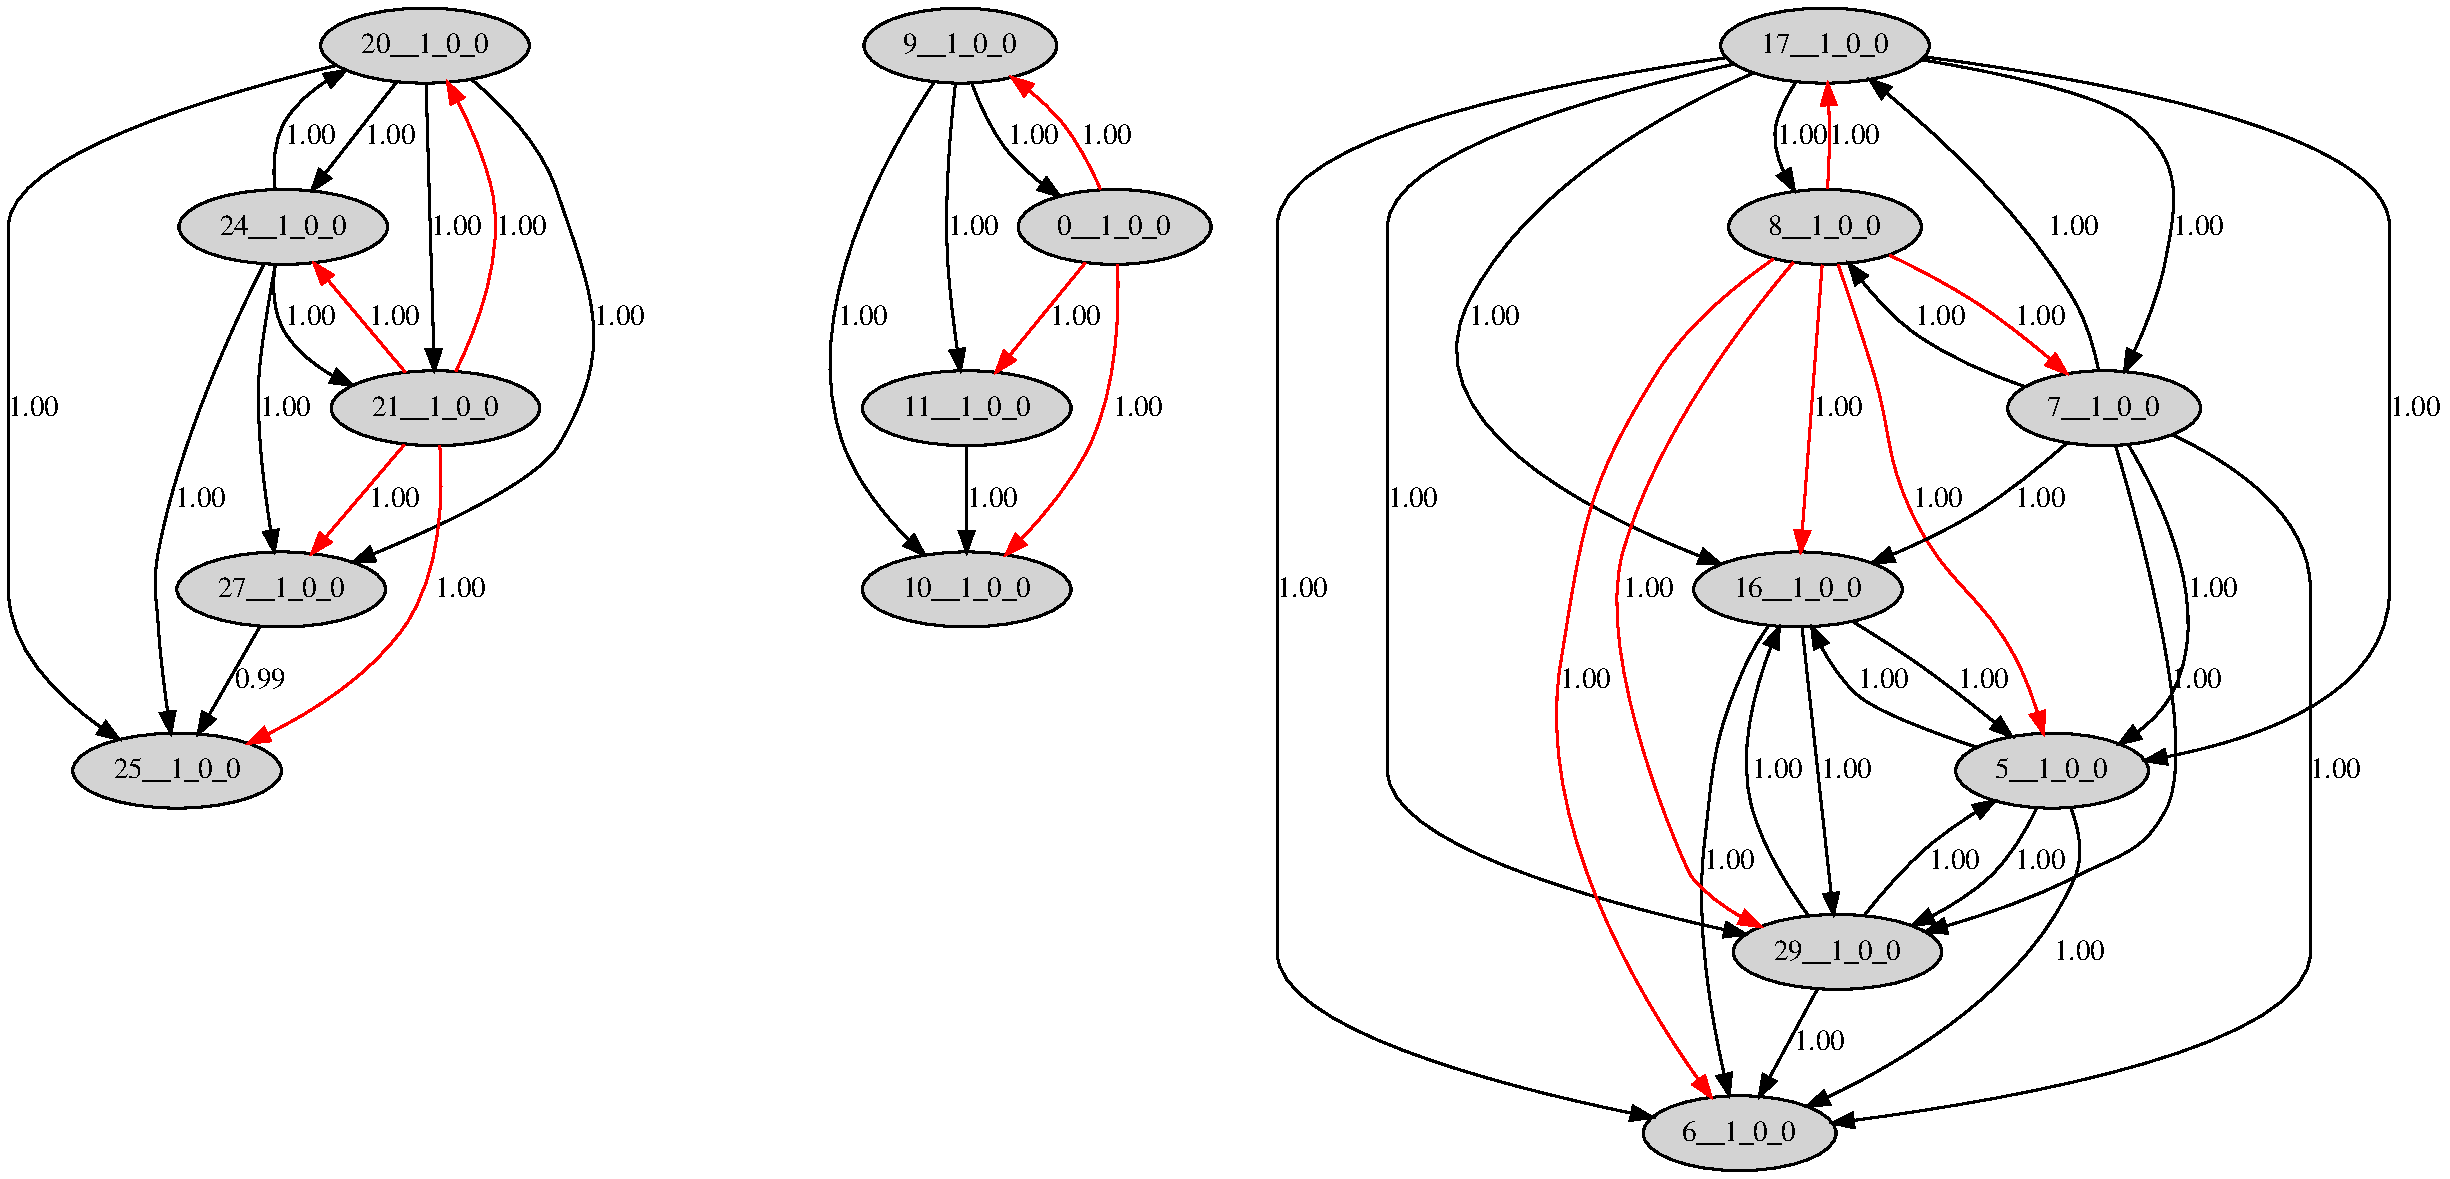
\includegraphics[width=0.88\linewidth]{YaleLanguages_1-s_1_l_0-graph.pdf}
  }
  \caption{\textit{YaleLanguages\_1} correlation graph}
  \label{fig:appendix:corrgraphs:yale}
\end{sidewaysfigure}

\begin{sidewaysfigure}[h]
  \centering
  \makebox[\textwidth][c]{
    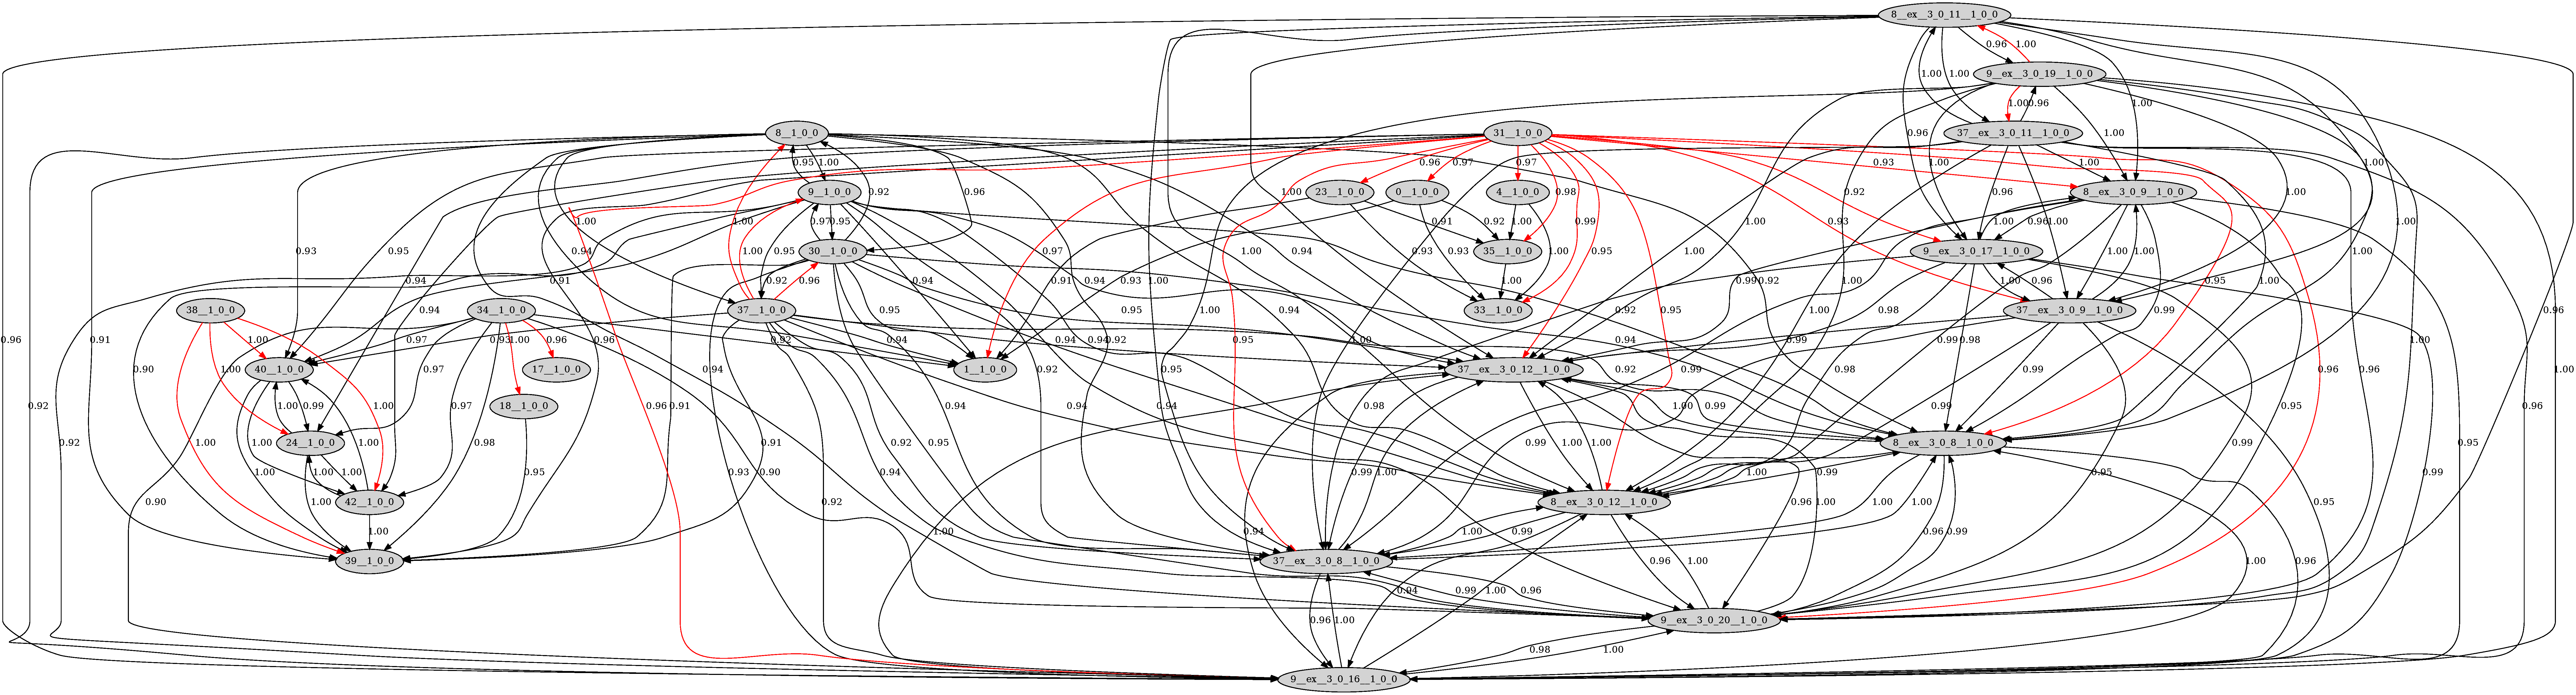
\includegraphics[width=1.08\linewidth]{Generico_1-corr-s_1_l_0-graph.pdf}
  }
  \caption{\textit{Generico\_1} correlation graph}
  \label{fig:appendix:corrgraphs:generico}
\end{sidewaysfigure}


% --------- notes --------- %

\iffalse
- interesting results:
  - correlation graphs \& heatmaps
  - pattern distribution
  - n-gram analysis
  - other plots that you already have
- concrete examples of whitebox representation of interesting columns (similar to the ones in presentation); with calculation of compression ratio, etc.
\fi

\iffalse
To better understand the impact of \textit{whitebox compression} and how it affects the compression ratio we selected \verb|todo| representative tables and analyzed their compression trees and size components. TODO-1: analyze 2-3 tables

analyze:
YaleLanguages - very good with both vw and wc, but small
Generico - large, decent with vw, significantly good with wb
Redfin1\_1 - not good overall, but good in used -> lack of compression opportunities
RealEstate2\_1 - not good with used either
\fi


% --------- end appendices --------- %

\end{appendices}

% ---------------------------------------------------------------------------
%: ----------------------- end of thesis sub-document ------------------------
% ---------------------------------------------------------------------------


      
            
% --------------------------------------------------------------
%:                  BACK MATTER: appendices, refs,..
% --------------------------------------------------------------

% the back matter: appendix and references close the thesis


%: ----------------------- bibliography ------------------------

% The section below defines how references are listed and formatted
% The default below is 2 columns, small font, complete author names.
% Entries are also linked back to the page number in the text and to external URL if provided in the BibTex file.

% PhDbiblio-url2 = names small caps, title bold & hyperlinked, link to page 
%\begin{multicols}{2} % \begin{multicols}{ # columns}[ header text][ space]
%\begin{tiny} % tiny(5) < scriptsize(7) < footnotesize(8) < small (9)

\bibliographystyle{Latex/Classes/PhDbiblio-url2} % Title is link if provided
\renewcommand{\bibname}{References} % changes the header; default: Bibliography

\bibliography{7_references/references} % adjust this to fit your BibTex file

%\end{tiny}
%\end{multicols}



% --------------------------------------------------------------
% Various bibliography styles exit. Replace above style as desired.

% in-text refs: (1) (1; 2)
% ref list: alphabetical; author(s) in small caps; initials last name; page(s)
%\bibliographystyle{Latex/Classes/PhDbiblio-case} % title forced lower case
%\bibliographystyle{Latex/Classes/PhDbiblio-bold} % title as in bibtex but bold
%\bibliographystyle{Latex/Classes/PhDbiblio-url} % bold + www link if provided

%\bibliographystyle{Latex/Classes/jmb} % calls style file jmb.bst
% in-text refs: author (year) without brackets
% ref list: alphabetical; author(s) in normal font; last name, initials; page(s)

%\bibliographystyle{plainnat} % calls style file plainnat.bst
% in-text refs: author (year) without brackets
% (this works with package natbib)


% --------------------------------------------------------------

% according to Dresden med fac summary has to be at the end
%
% Thesis Abstract -----------------------------------------------------


%\begin{abstractslong}    %uncommenting this line, gives a different abstract heading
\begin{abstracts}        %this creates the heading for the abstract page

Existing columnar database systems rely on a small set of lightweight compression techniques to achieve smaller data size and fast query execution: RLE, DICT, FOR, DELTA and their improved versions. These are hardcoded blackbox approaches with limited capacity of exploiting all compression opportunities present in real data. We propose \textit{whitebox compression}: a new compression model which represents data through elementary operator expressions automatically generated at bulk load. This is done by learning patterns from the data and associating them with operators to form expression trees, which are stored together with the compressed data and lazily evaluated during query execution. \textit{Whitebox compression} automatically finds and exploits compression opportunities, leading to transparent, recursive and more compact representations of the data. Combined with vectorized execution or JIT code generation, it has the potential to generate powerful compression schemes in terms of both compression ratio and query execution time. Our focus is on real data rather than synthetic datasets, thus we develop and evaluate the \textit{whitebox compression} model using the Public BI benchmark---a comprehensive human generated benchmark for database systems.
\end{abstracts}
%\end{abstractlongs}


% ---------------------------------------------------------------------- 


%: Declaration of originality
%\include{8_backmatter/declaration}



\end{document}
